\section{Provided Test Cases}
In this section, we provide the output wave for the provided test cases. We show both full code results and the results of disabled hazard handling. Also, we show the wave of handling hazards through NOPs.

\subsection{One Operand Test Case}

\subsubsection{Full Code}
The figures \ref{fig:1op_reg_1} and \ref{fig:1op_reg_2} show the output wave of full code.
\begin{figure}[H]
    \centering
    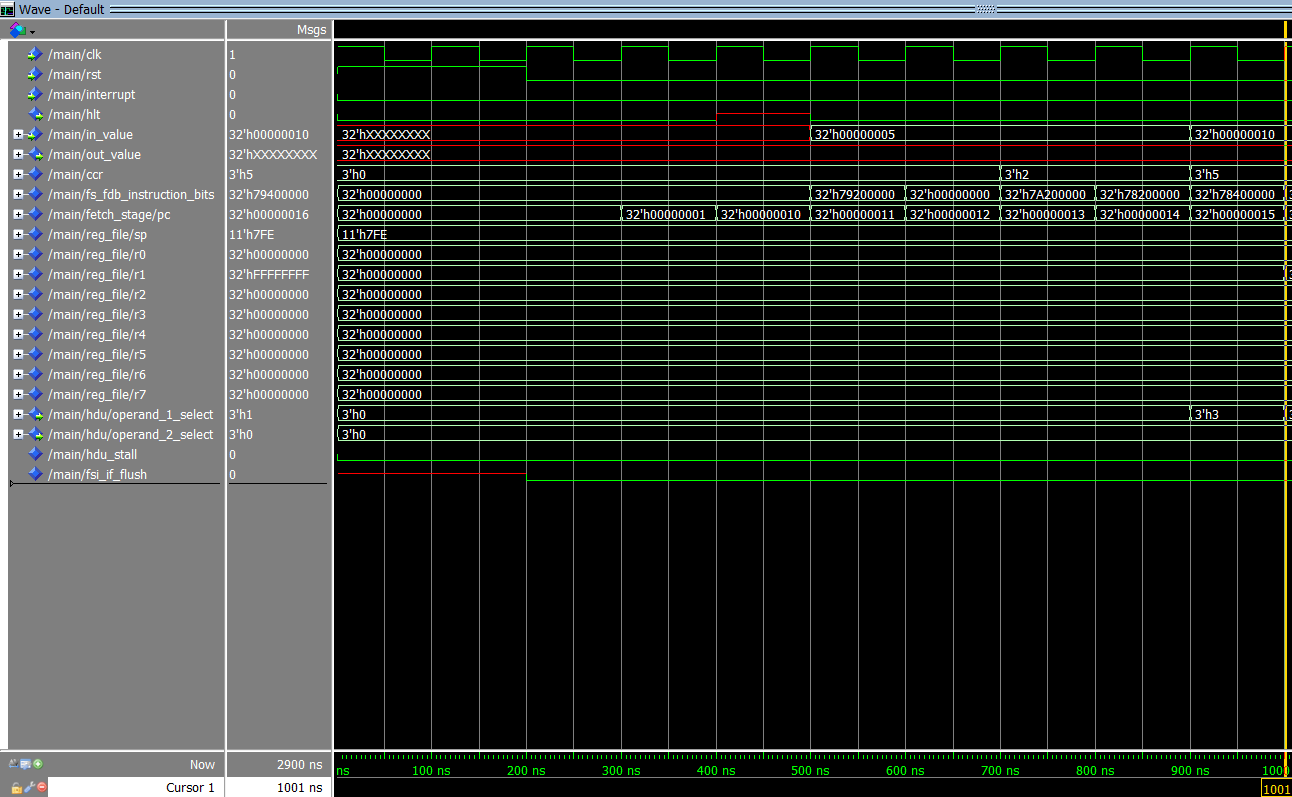
\includegraphics[width=0.9\textwidth]{images/test_cases/one_operand/OneOperand_regular_1.PNG}
    \caption{One Operand Full Code Output wave 1}
    \label{fig:1op_reg_1}
\end{figure}

\begin{figure}[H]
    \centering
    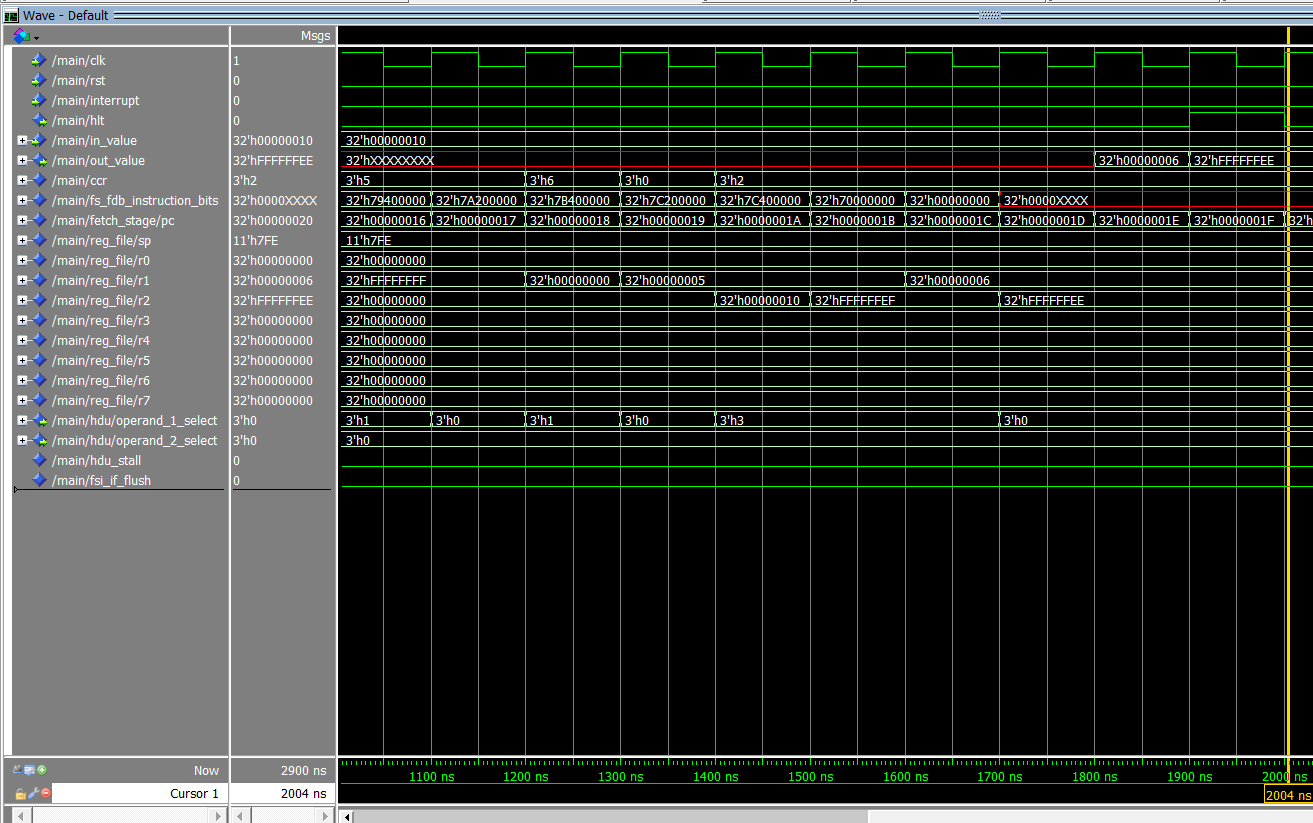
\includegraphics[width=0.9\textwidth]{images/test_cases/one_operand/OneOperand_regular_2.PNG}
    \caption{One Operand Full Code Output wave 2}
    \label{fig:1op_reg_2}
\end{figure}

\subsubsection{No Forwarding}
The figures \ref{fig:1op_no_1} and \ref{fig:1op_no_2} show the output wave of code with no forwarding.
\begin{figure}[H]
    \centering
    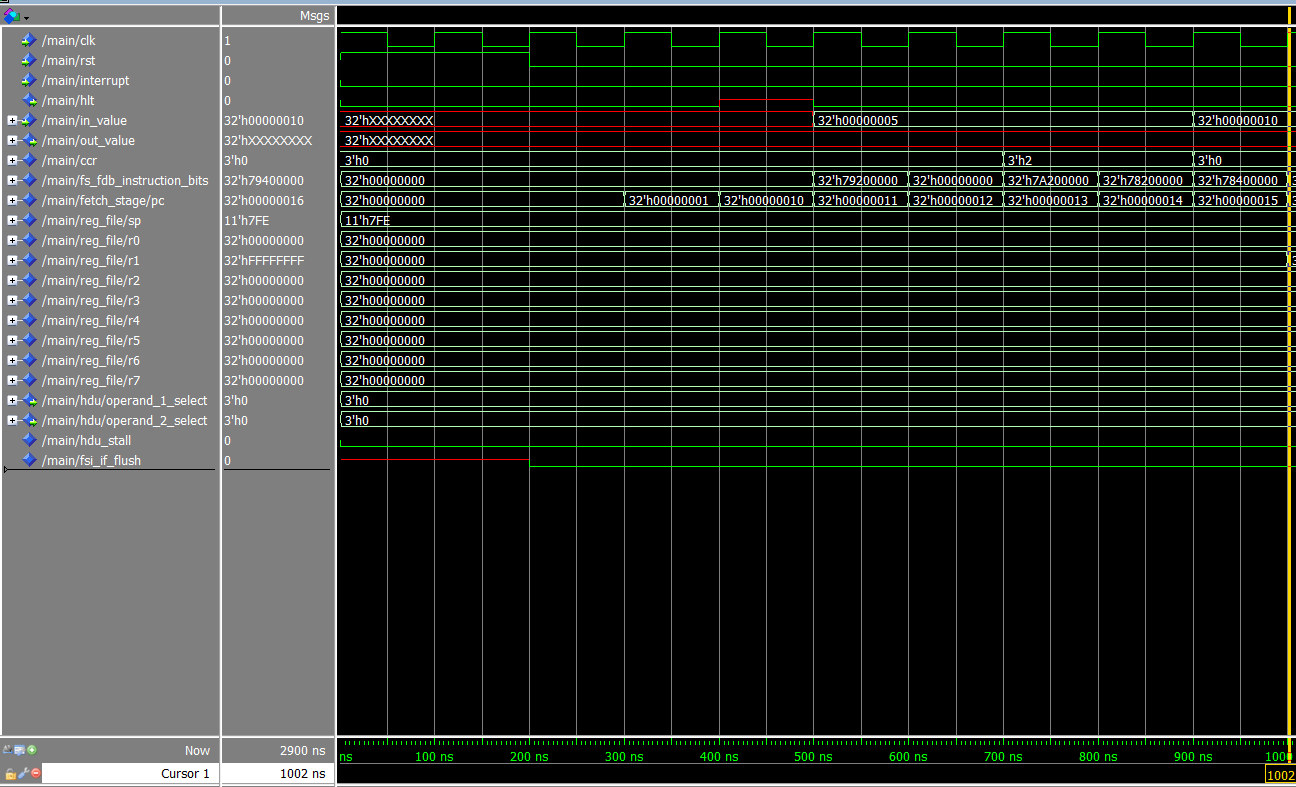
\includegraphics[width=0.9\textwidth]{images/test_cases/one_operand/OneOperand_no_forward_1.PNG}
    \caption{One Operand No Forwarding Output wave 1}
    \label{fig:1op_no_1}
\end{figure}

\begin{figure}[H]
    \centering
    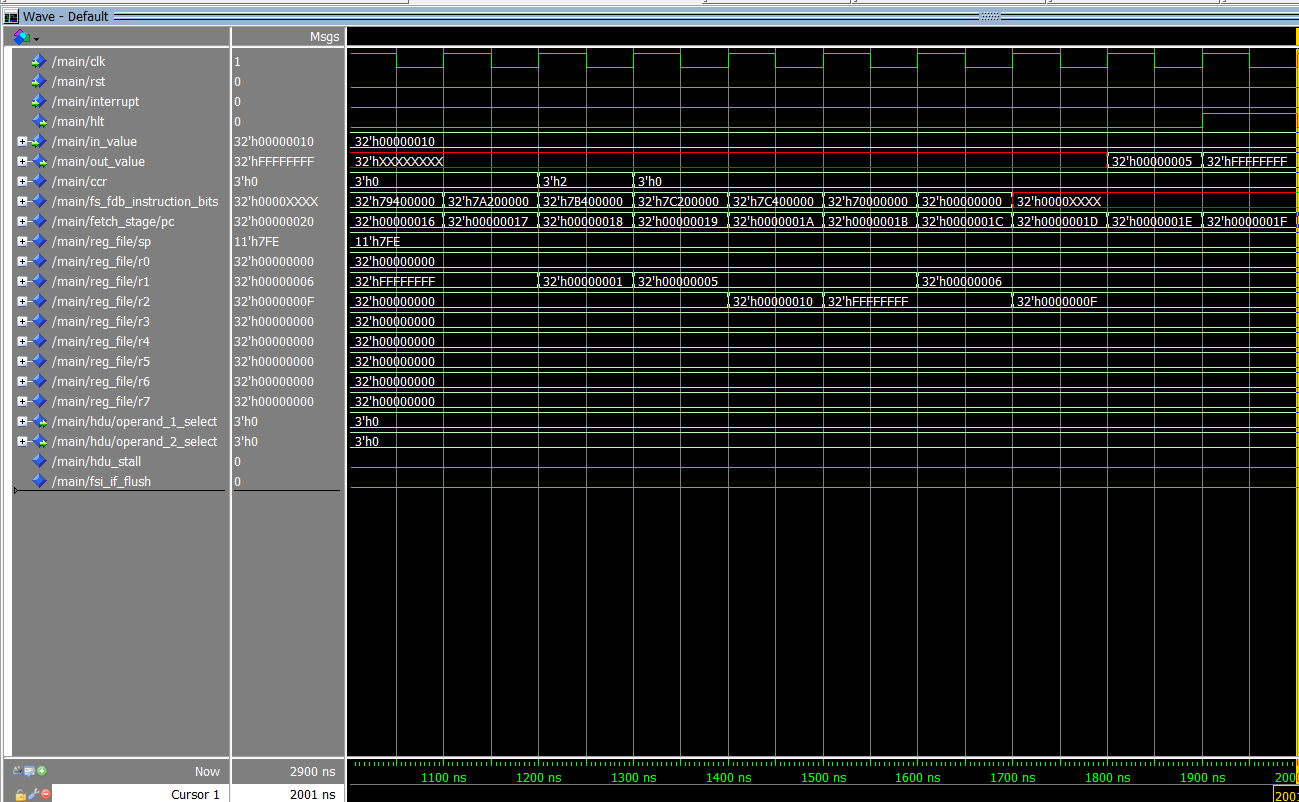
\includegraphics[width=0.9\textwidth]{images/test_cases/one_operand/OneOperand_no_forward_2.PNG}
    \caption{One Operand No Forwarding Output wave 2}
    \label{fig:1op_no_2}
\end{figure}

\subsubsection{NOPs Solution}
The figures \ref{fig:1op_nop_1}, \ref{fig:1op_nop_2} and \ref{fig:1op_nop_3} show the output wave of code with NOPs solution.
\begin{figure}[H]
    \centering
    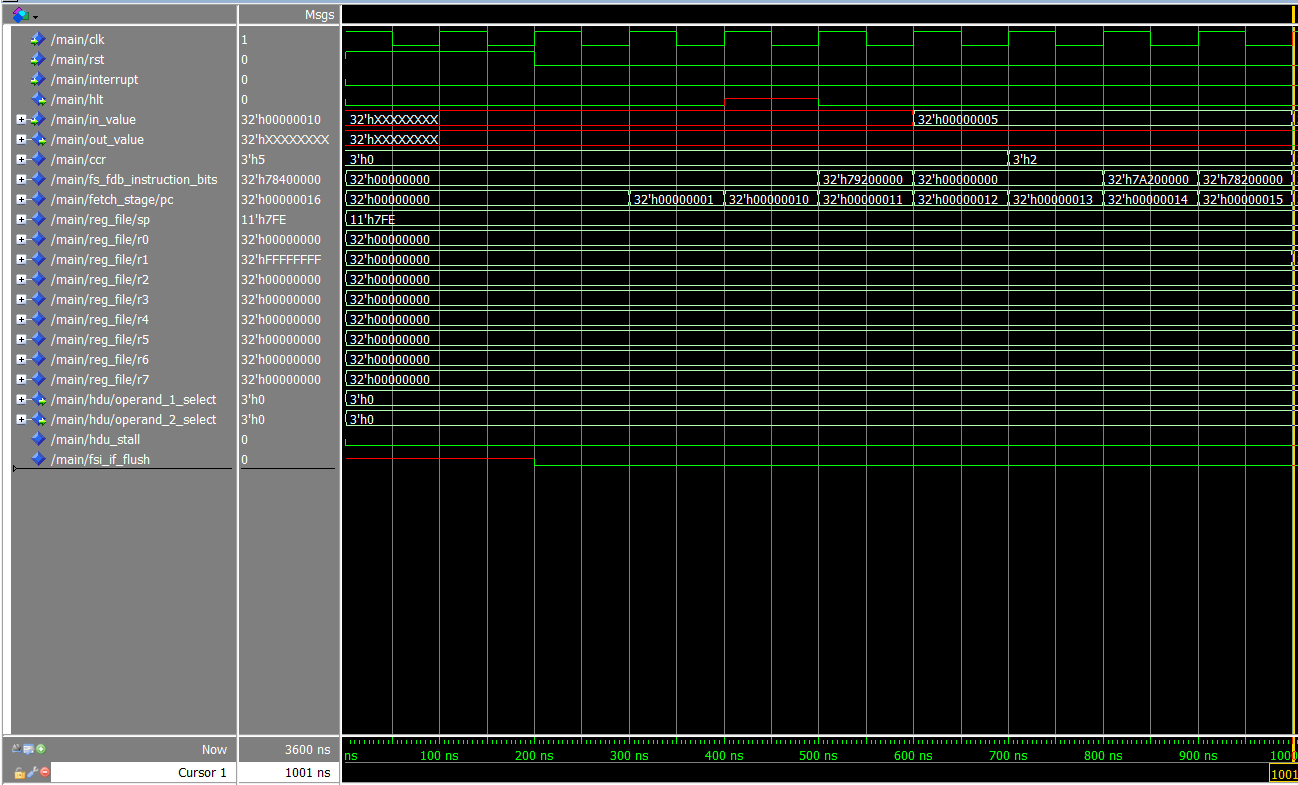
\includegraphics[width=0.9\textwidth]{images/test_cases/one_operand/OneOperand_NOP_1.PNG}
    \caption{One Operand NOPs Solution Output wave 1}
    \label{fig:1op_nop_1}
\end{figure}

\begin{figure}[H]
    \centering
    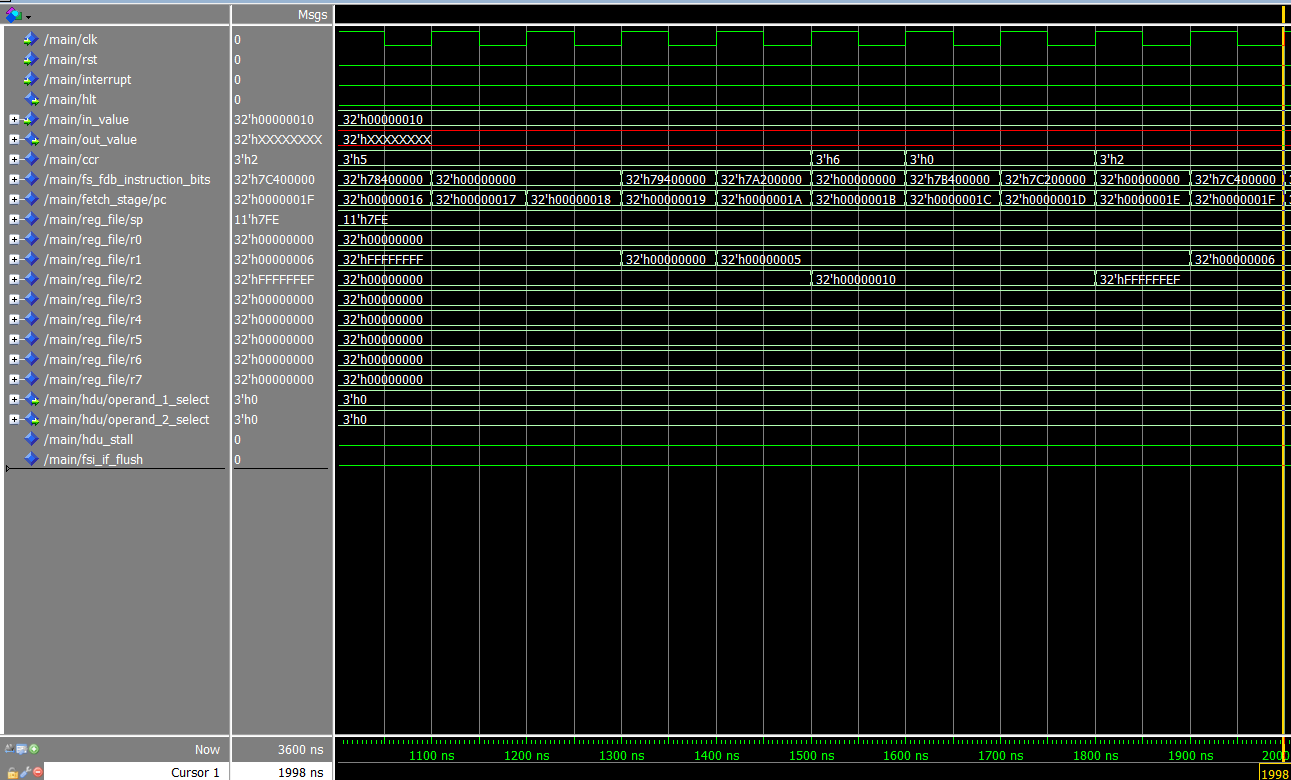
\includegraphics[width=0.9\textwidth]{images/test_cases/one_operand/OneOperand_NOP_2.PNG}
    \caption{One Operand NOPs Solution Output wave 2}
    \label{fig:1op_nop_2}
\end{figure}

\begin{figure}[H]
    \centering
    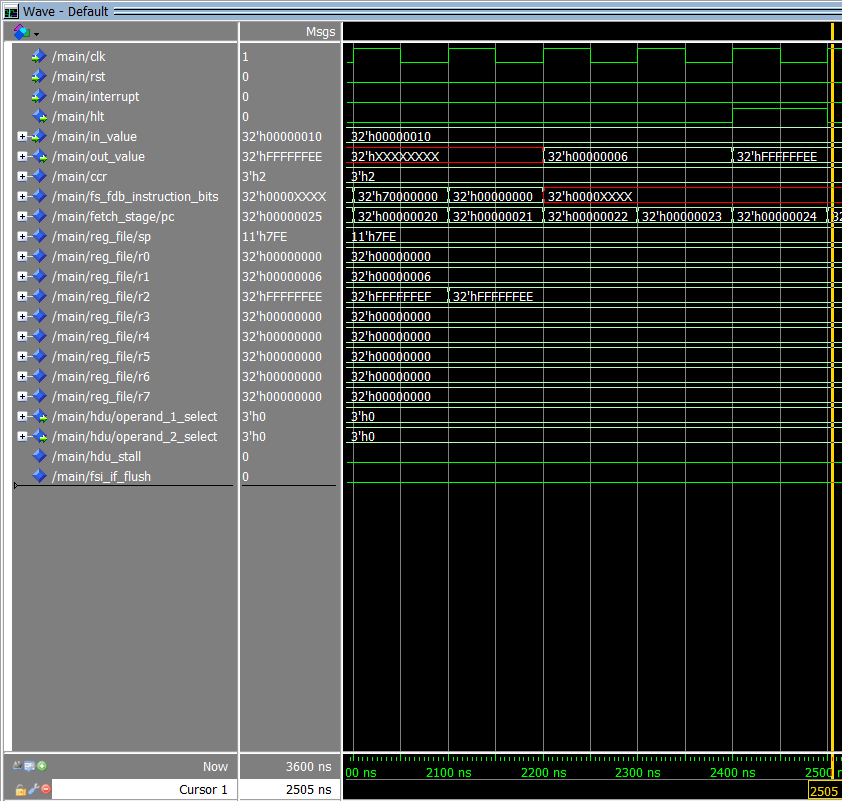
\includegraphics[width=0.9\textwidth]{images/test_cases/one_operand/OneOperand_NOP_3.PNG}
    \caption{One Operand NOPs Solution Output wave 3}
    \label{fig:1op_nop_3}
\end{figure}


\subsection{Two Operand Test Case}

\subsubsection{Full Code}
The figures \ref{fig:2op_reg_1}, \ref{fig:2op_reg_2} and \ref{fig:2op_reg_3} show the output wave of full code.
\begin{figure}[H]
    \centering
    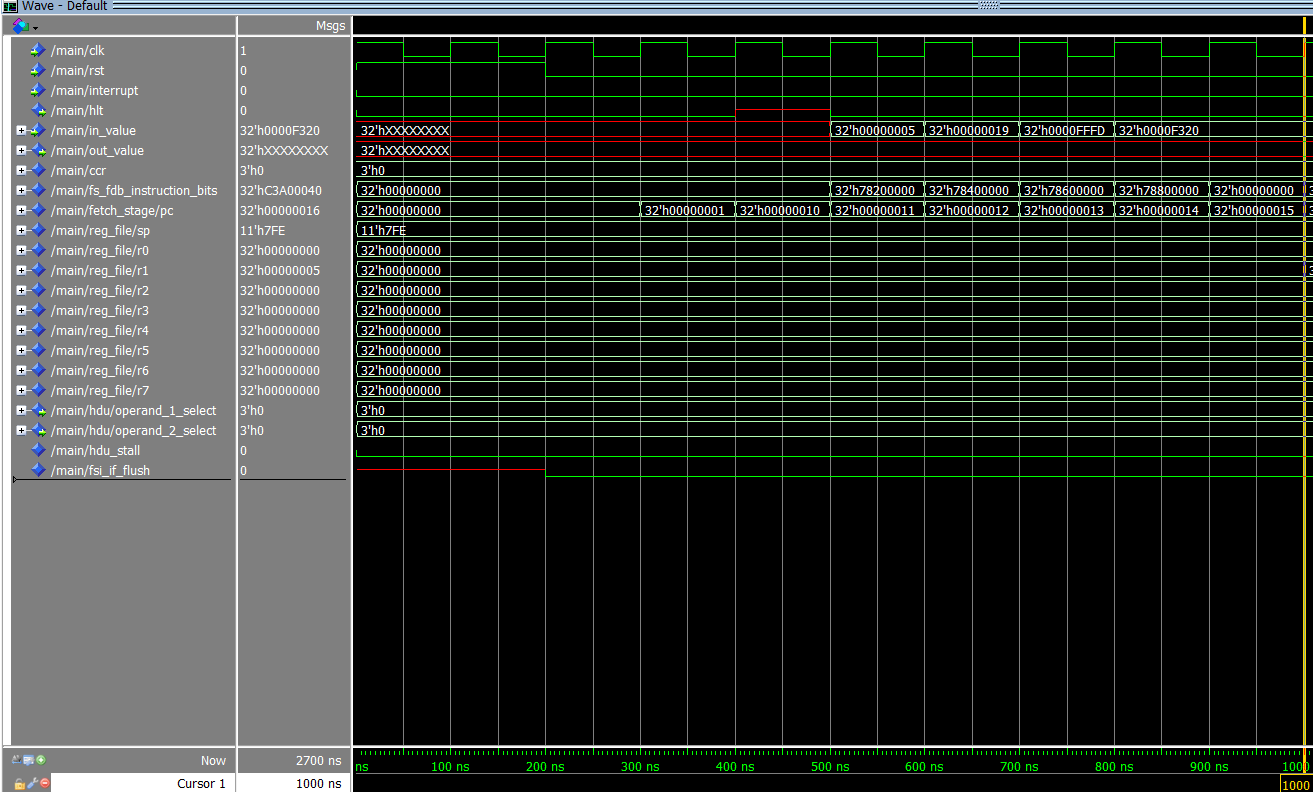
\includegraphics[width=0.9\textwidth]{images/test_cases/two_operand/TwoOperand_regular_1.PNG}
    \caption{Two Operand Full Code Output wave 1}
    \label{fig:2op_reg_1}
\end{figure}

\begin{figure}[H]
    \centering
    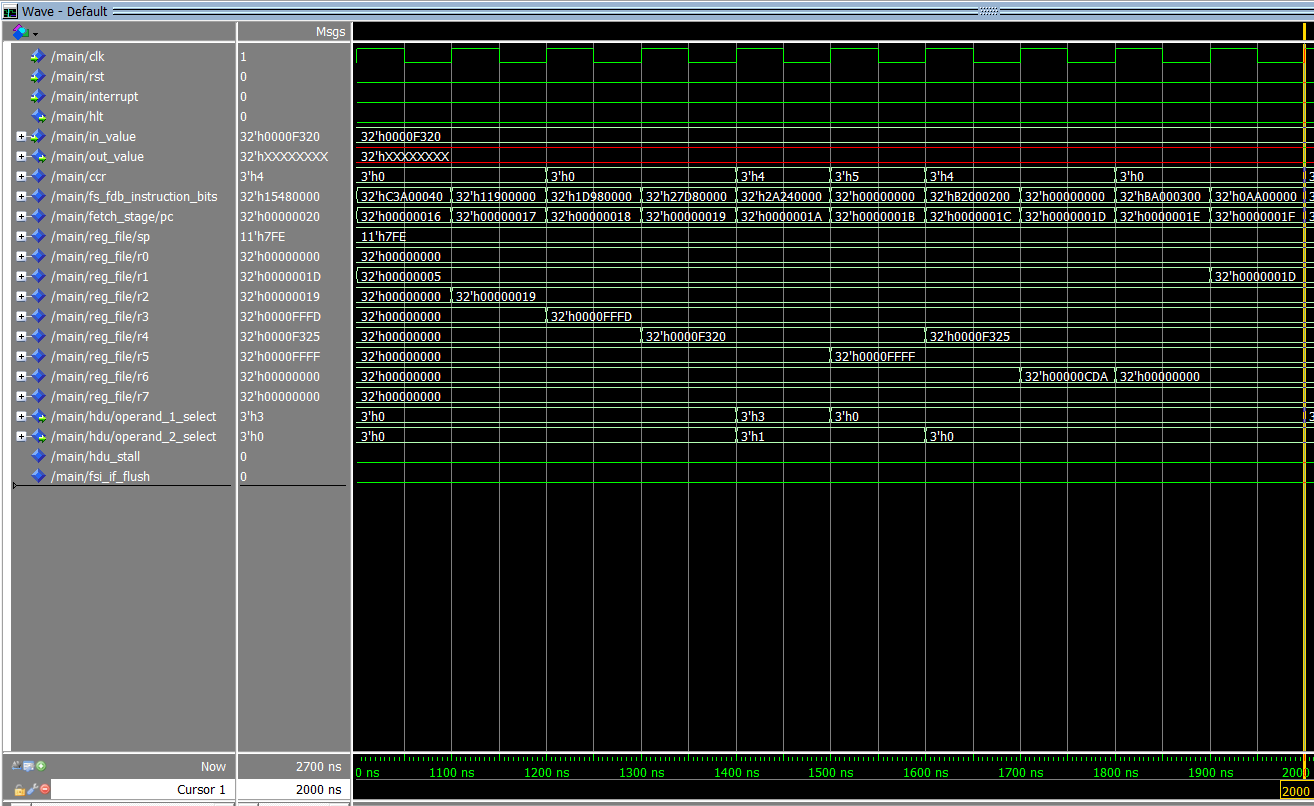
\includegraphics[width=0.9\textwidth]{images/test_cases/two_operand/TwoOperand_regular_2.PNG}
    \caption{Two Operand Full Code Output wave 2}
    \label{fig:2op_reg_2}
\end{figure}

\begin{figure}[H]
    \centering
    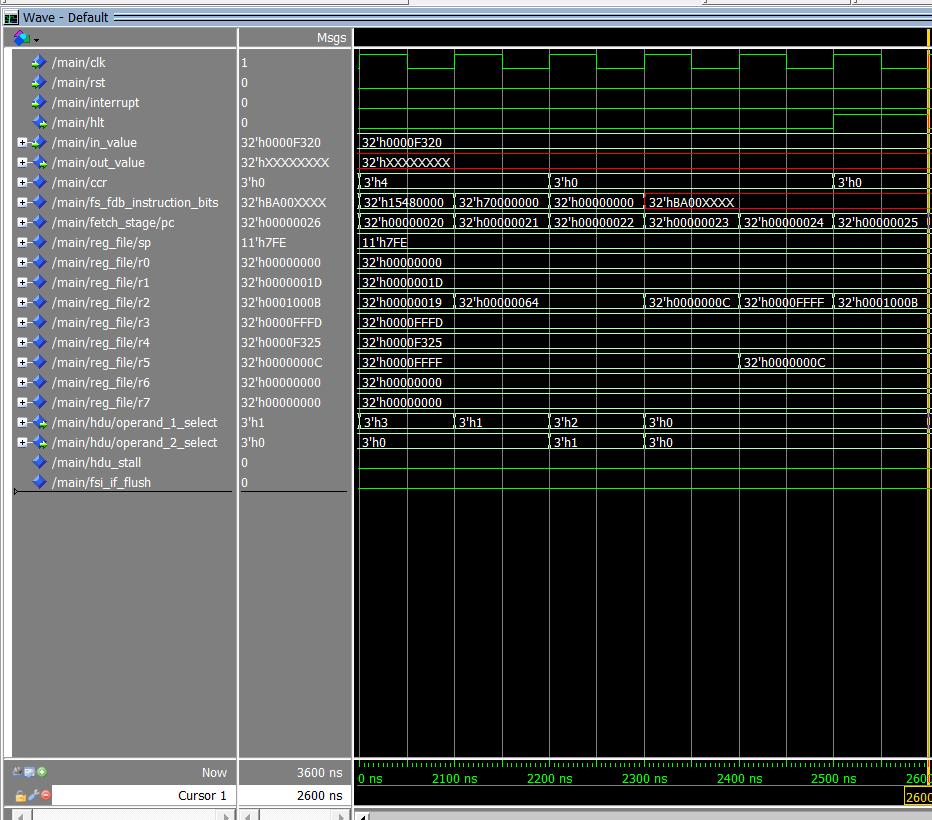
\includegraphics[width=0.9\textwidth]{images/test_cases/two_operand/TwoOperand_regular_3.PNG}
    \caption{Two Operand Full Code Output wave 3}
    \label{fig:2op_reg_3}
\end{figure}

\subsubsection{No Forwarding}
The figures \ref{fig:2op_no_1}, \ref{fig:2op_no_2} and \ref{fig:2op_no_3} show the output wave of code with no forwarding.
\begin{figure}[H]
    \centering
    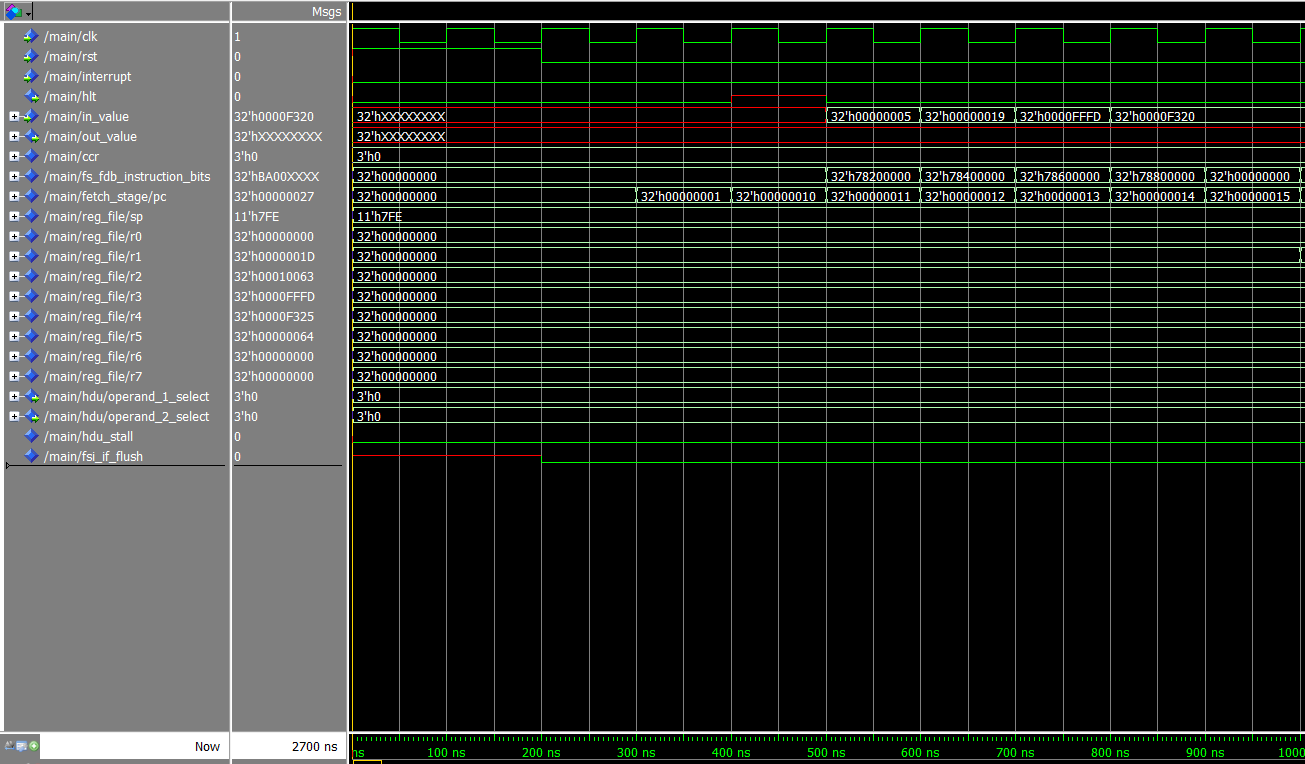
\includegraphics[width=0.9\textwidth]{images/test_cases/two_operand/TwoOperand_no_forward_1.PNG}
    \caption{Two Operand No Forwarding Output wave 1}
    \label{fig:2op_no_1}
\end{figure}

\begin{figure}[H]
    \centering
    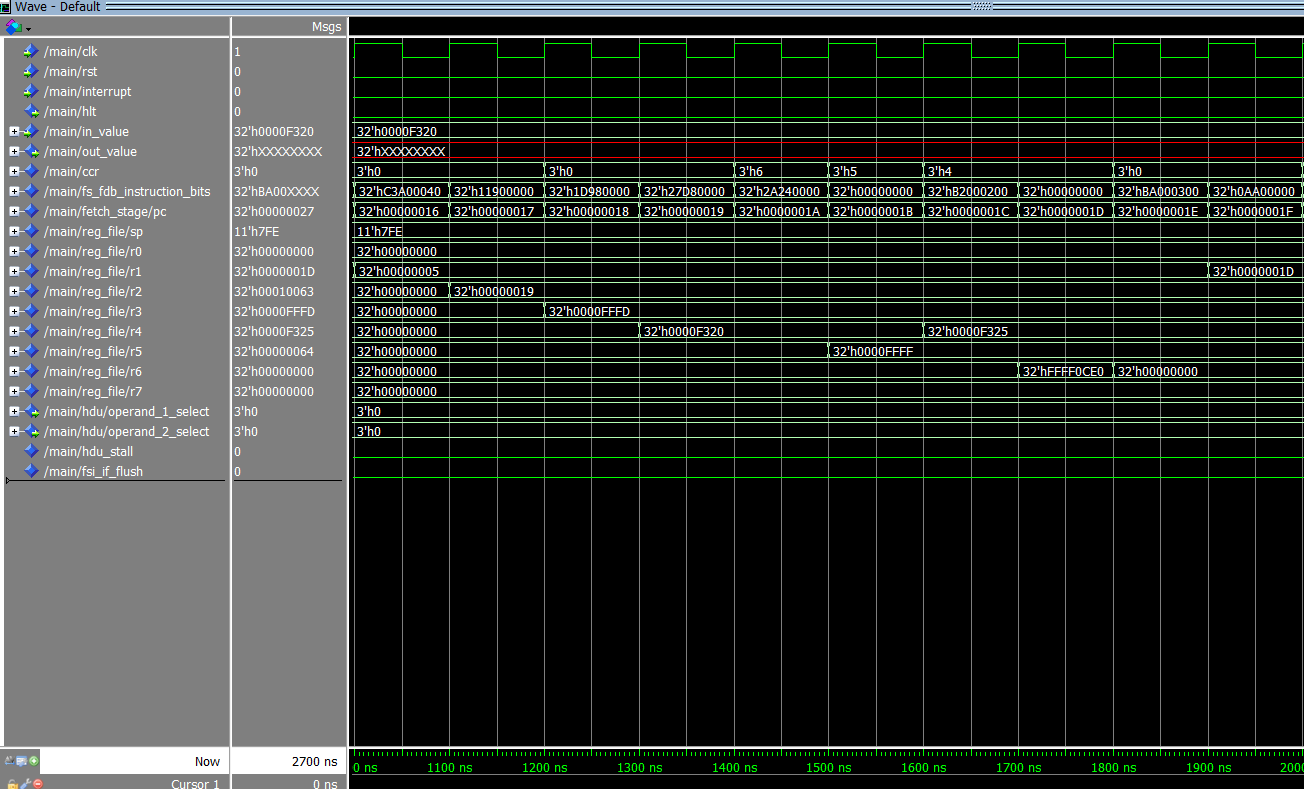
\includegraphics[width=0.9\textwidth]{images/test_cases/two_operand/TwoOperand_no_forward_2.PNG}
    \caption{Two Operand No Forwarding Output wave 2}
    \label{fig:2op_no_2}
\end{figure}

\begin{figure}[H]
    \centering
    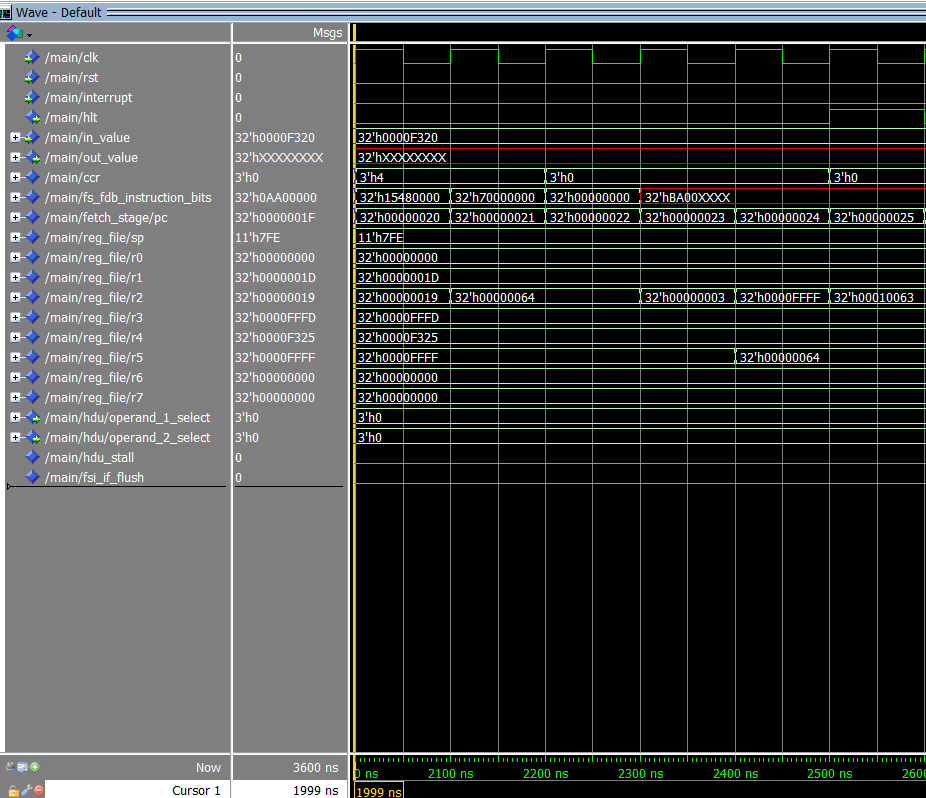
\includegraphics[width=0.9\textwidth]{images/test_cases/two_operand/TwoOperand_no_forward_3.PNG}
    \caption{Two Operand No Forwarding Output wave 3}
    \label{fig:2op_no_3}
\end{figure}

\subsubsection{NOPs Solution}
The figures \ref{fig:2op_nop_1}, \ref{fig:2op_nop_2}, \ref{fig:2op_nop_3} and \ref{fig:2op_nop_4} show the output wave of code with NOPs solution.
\begin{figure}[H]
    \centering
    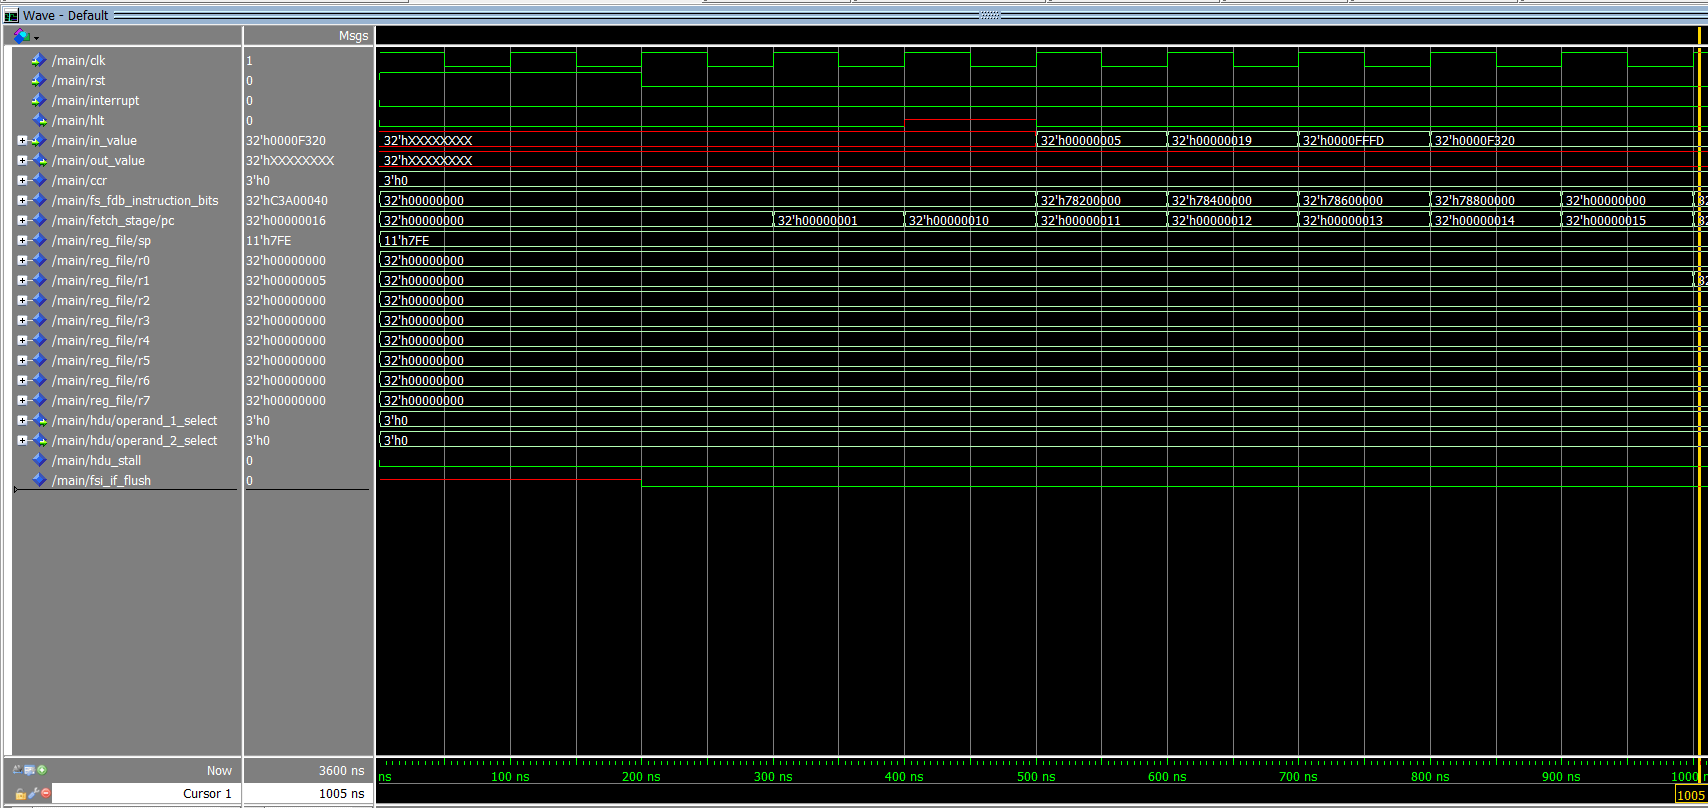
\includegraphics[width=0.9\textwidth]{images/test_cases/two_operand/TwoOperand_NOP_1.PNG}
    \caption{Two Operand NOPs Solution Output wave 1}
    \label{fig:2op_nop_1}
\end{figure}

\begin{figure}[H]
    \centering
    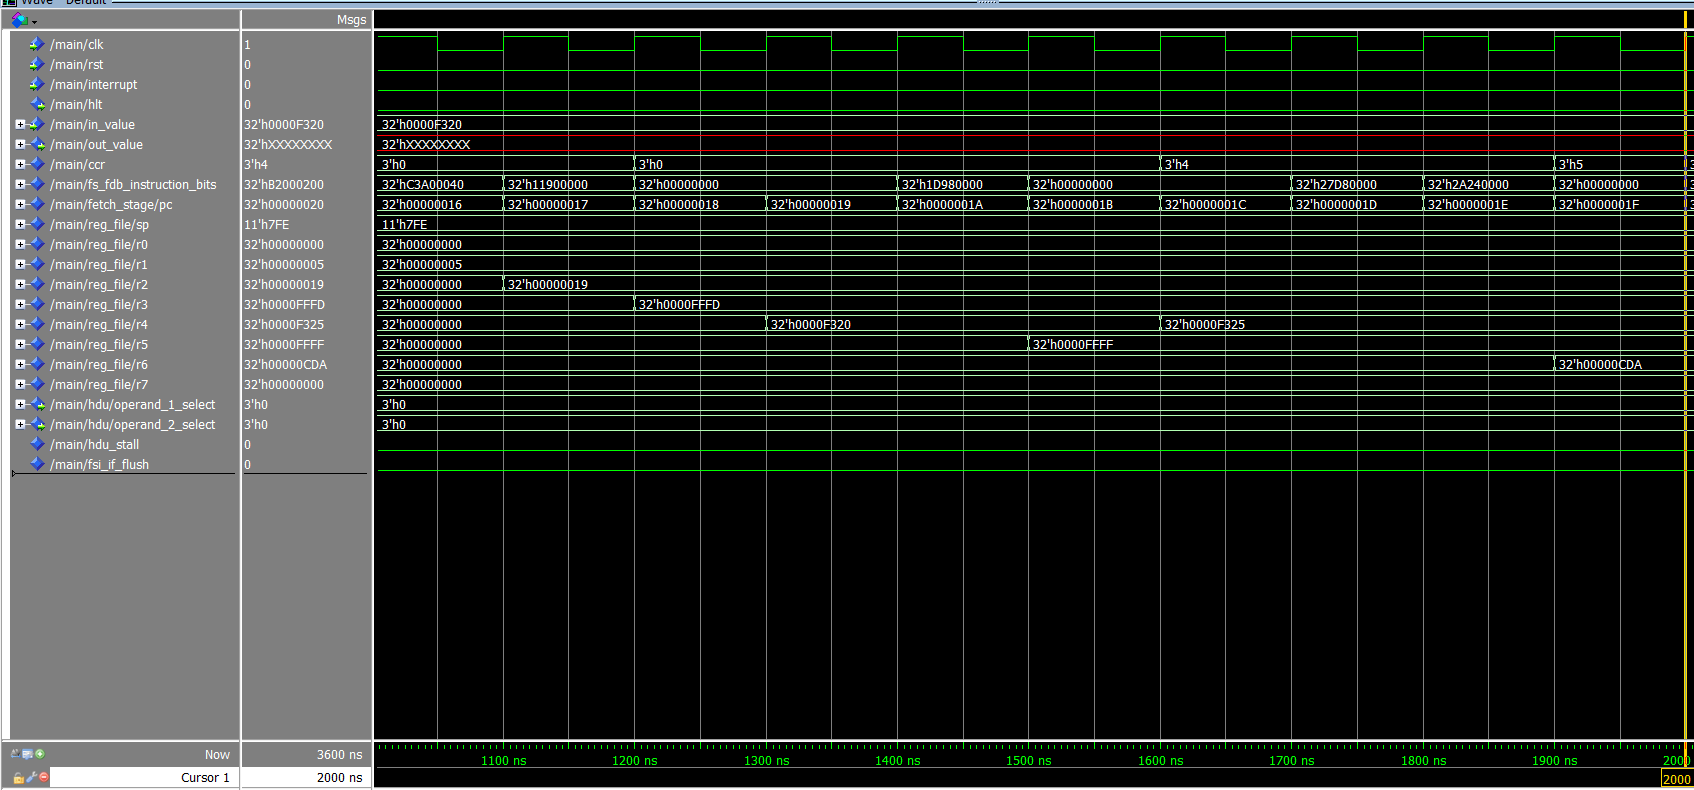
\includegraphics[width=0.9\textwidth]{images/test_cases/two_operand/TwoOperand_NOP_2.PNG}
    \caption{Two Operand NOPs Solution Output wave 2}
    \label{fig:2op_nop_2}
\end{figure}

\begin{figure}[H]
    \centering
    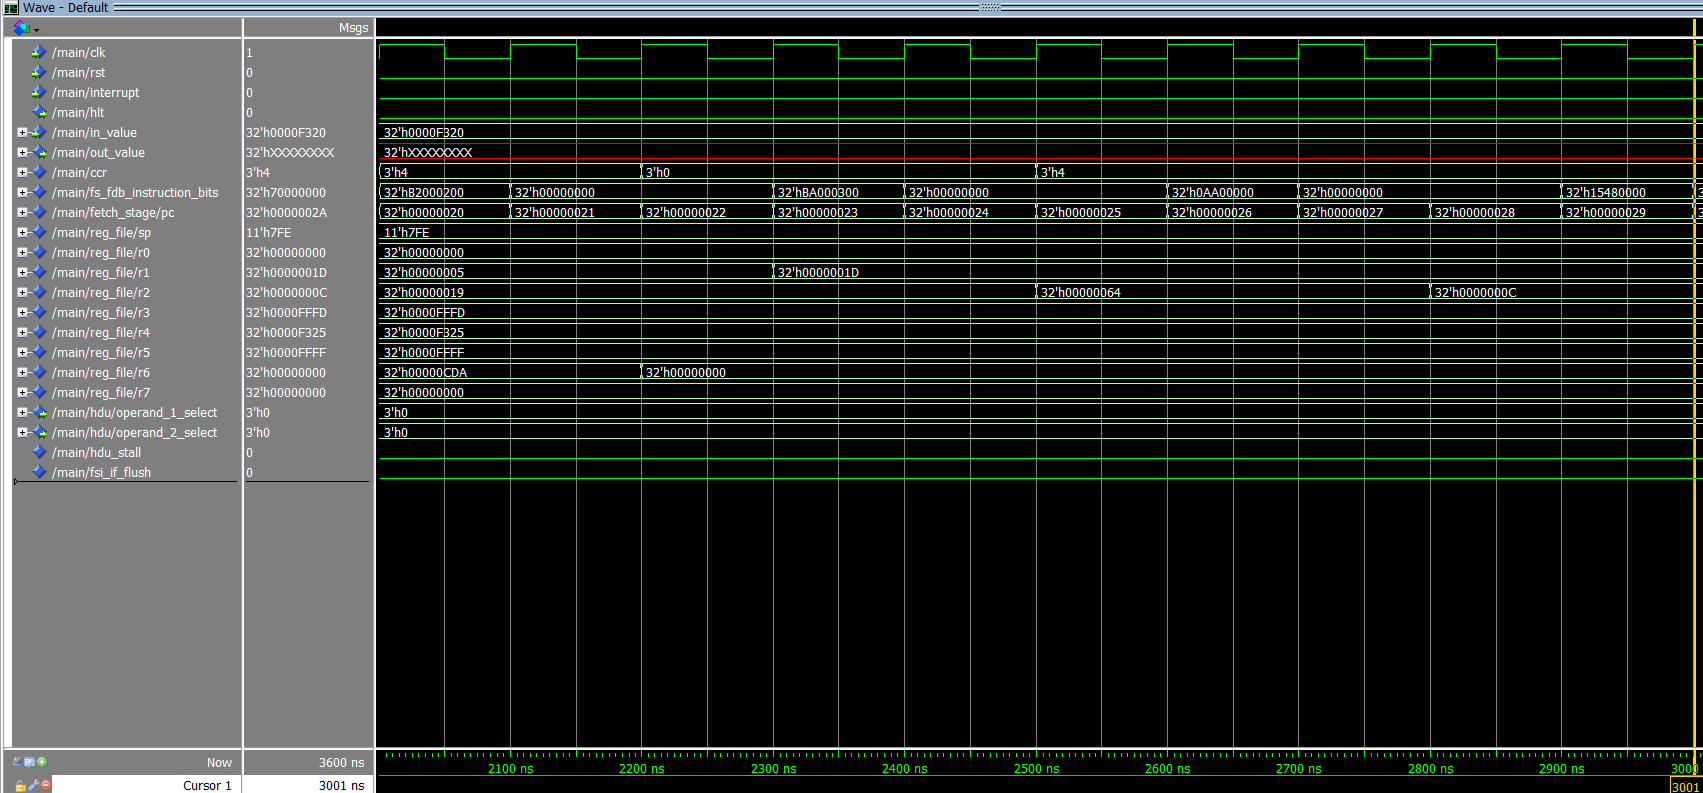
\includegraphics[width=0.9\textwidth]{images/test_cases/two_operand/TwoOperand_NOP_3.PNG}
    \caption{Two Operand NOPs Solution Output wave 3}
    \label{fig:2op_nop_3}
\end{figure}

\begin{figure}[H]
    \centering
    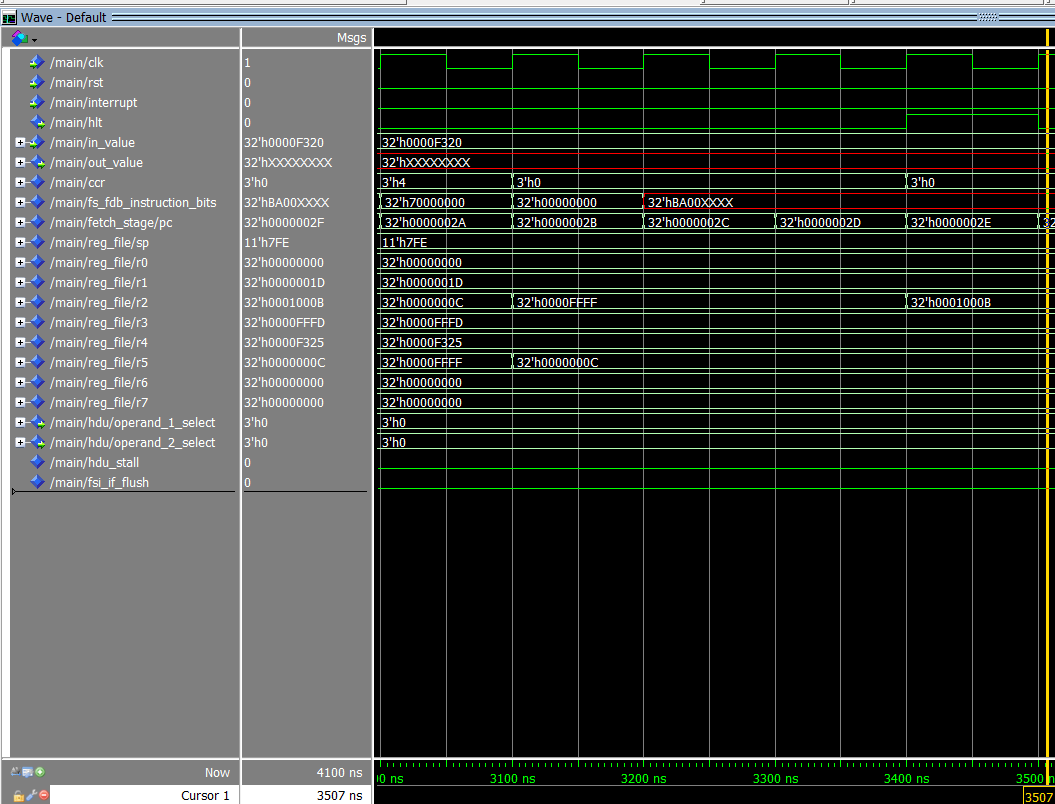
\includegraphics[width=0.9\textwidth]{images/test_cases/two_operand/TwoOperand_NOP_4.PNG}
    \caption{Two Operand NOPs Solution Output wave 4}
    \label{fig:2op_nop_4}
\end{figure}

\subsection{Memory Test Case}

\subsubsection{Full Code}
The figures \ref{fig:mem_reg_1}, \ref{fig:mem_reg_2} and \ref{fig:mem_reg_3} show the output wave of full code.
\begin{figure}[H]
    \centering
    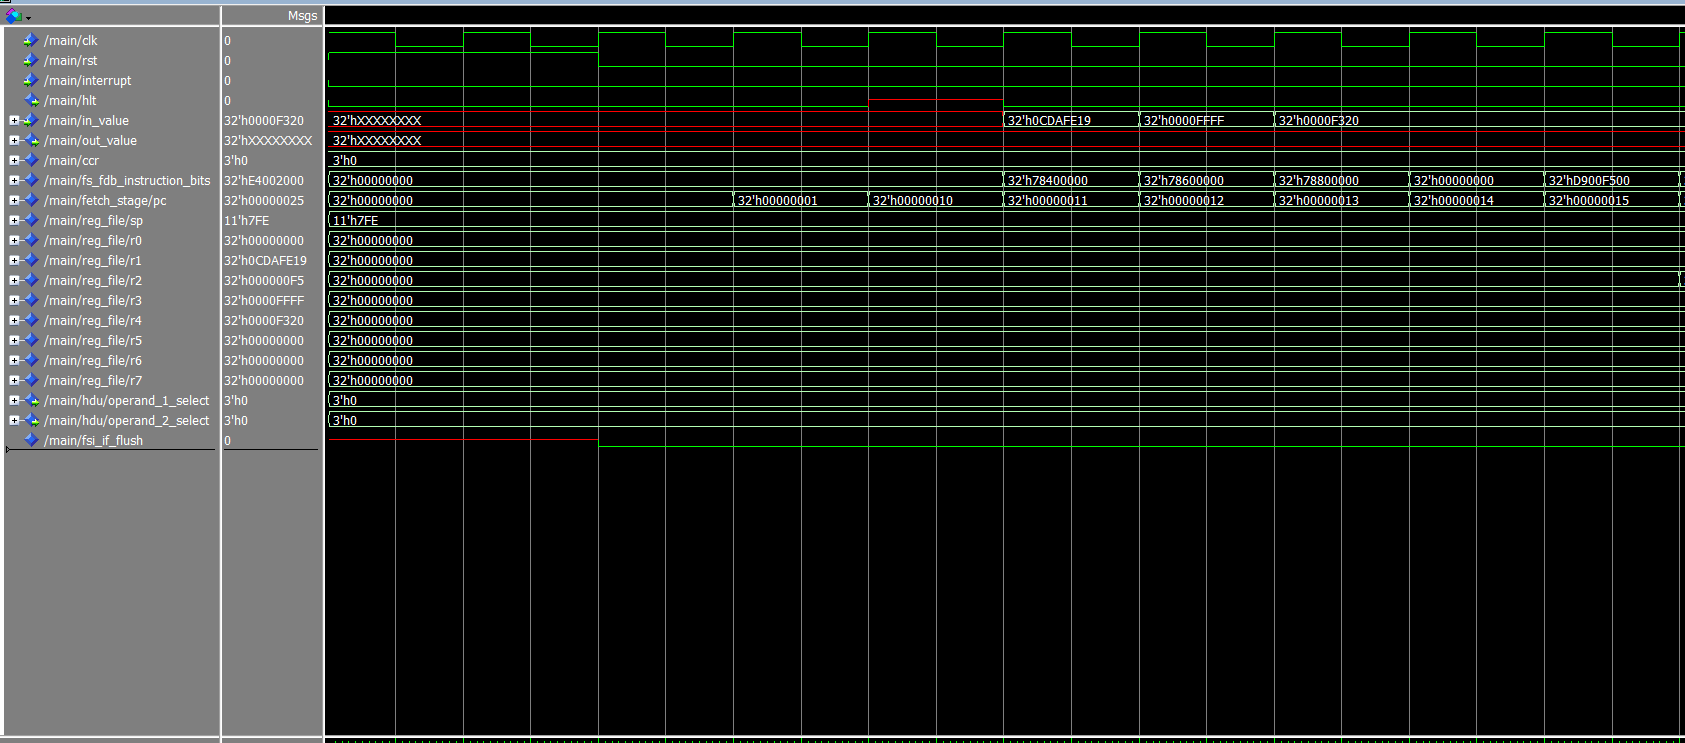
\includegraphics[width=0.9\textwidth]{images/test_cases/memory/Memory_regular_1.PNG}
    \caption{Memory Full Code Output wave 1}
    \label{fig:mem_reg_1}
\end{figure}

\begin{figure}[H]
    \centering
    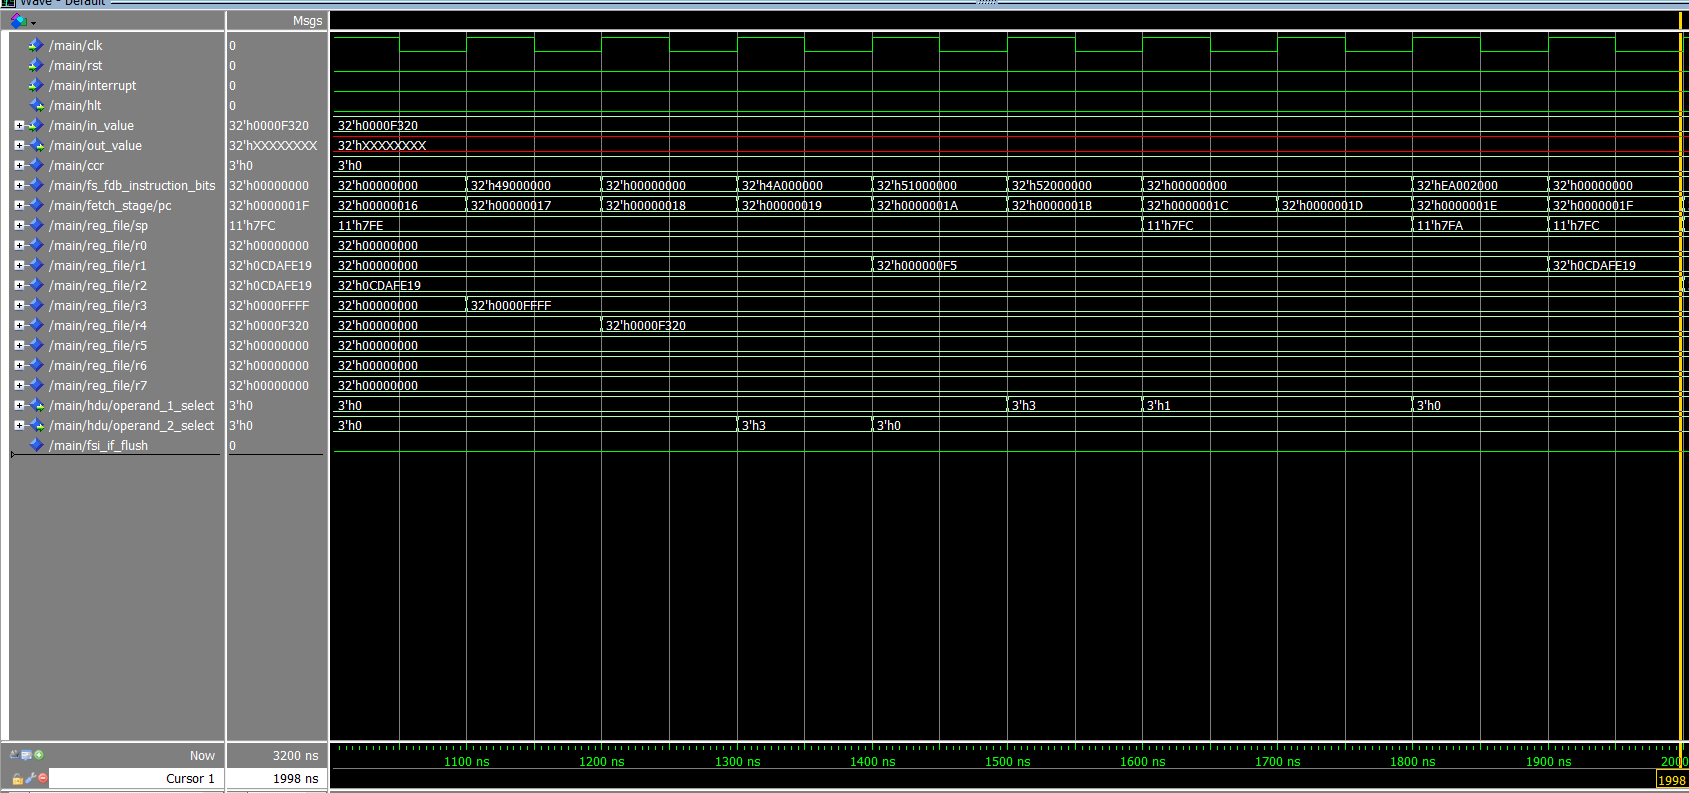
\includegraphics[width=0.9\textwidth]{images/test_cases/memory/Memory_regular_2.PNG}
    \caption{Memory Full Code Output wave 2}
    \label{fig:mem_reg_2}
\end{figure}

\begin{figure}[H]
    \centering
    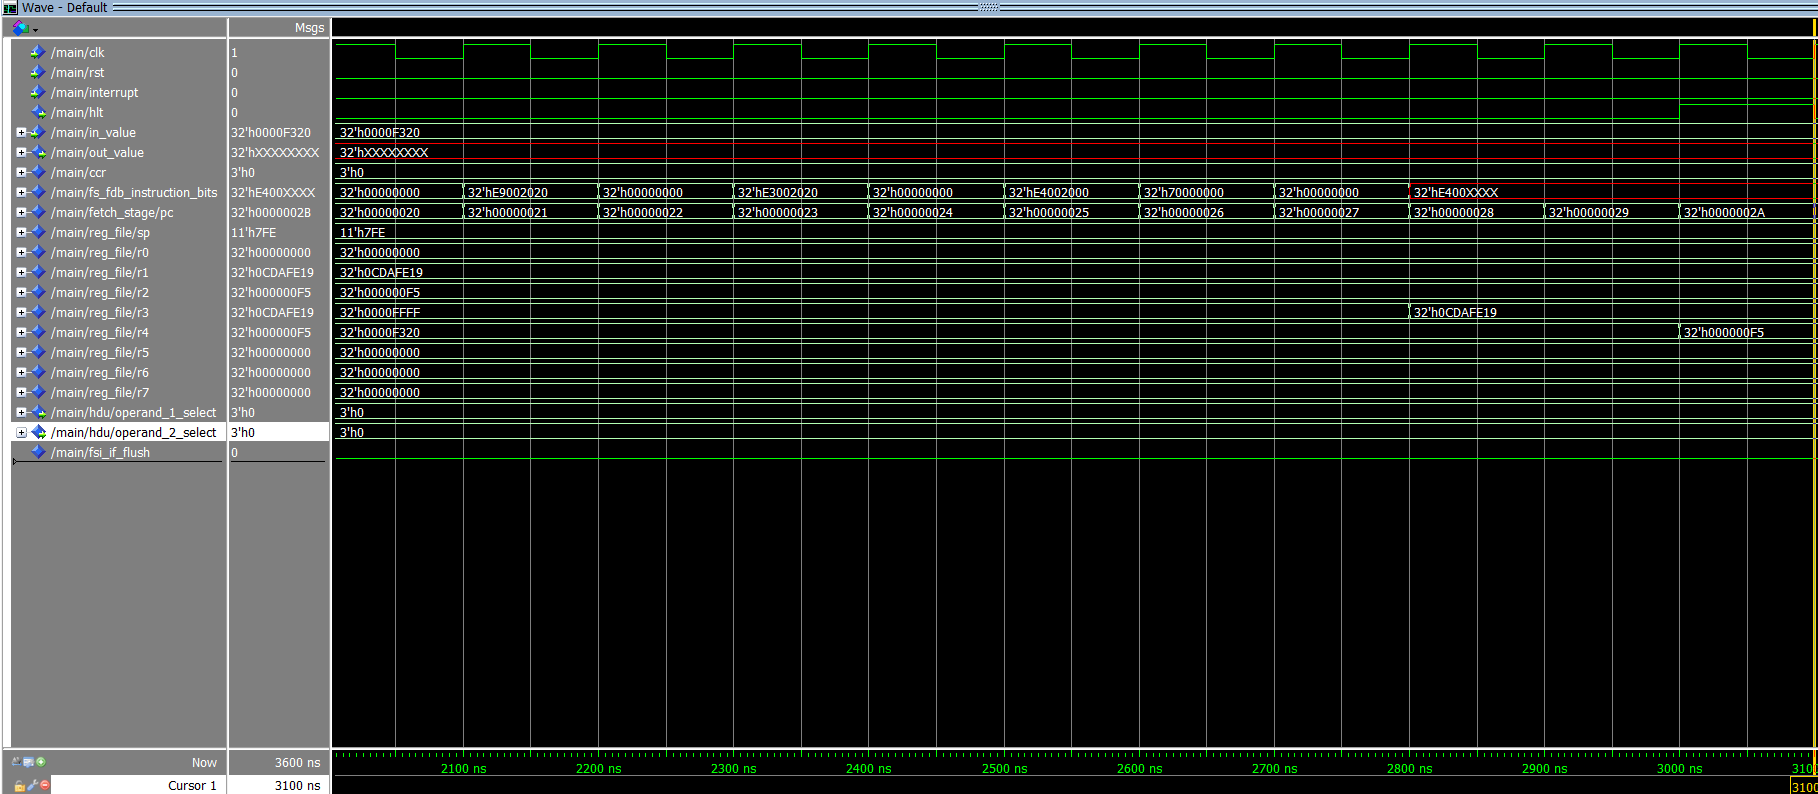
\includegraphics[width=0.9\textwidth]{images/test_cases/memory/Memory_regular_3.PNG}
    \caption{Memory Full Code Output wave 3}
    \label{fig:mem_reg_3}
\end{figure}

\subsubsection{No Forwarding}
The figures \ref{fig:mem_no_1}, \ref{fig:mem_no_2} and \ref{fig:mem_no_3} show the output wave of code with no forwarding.
\begin{figure}[H]
    \centering
    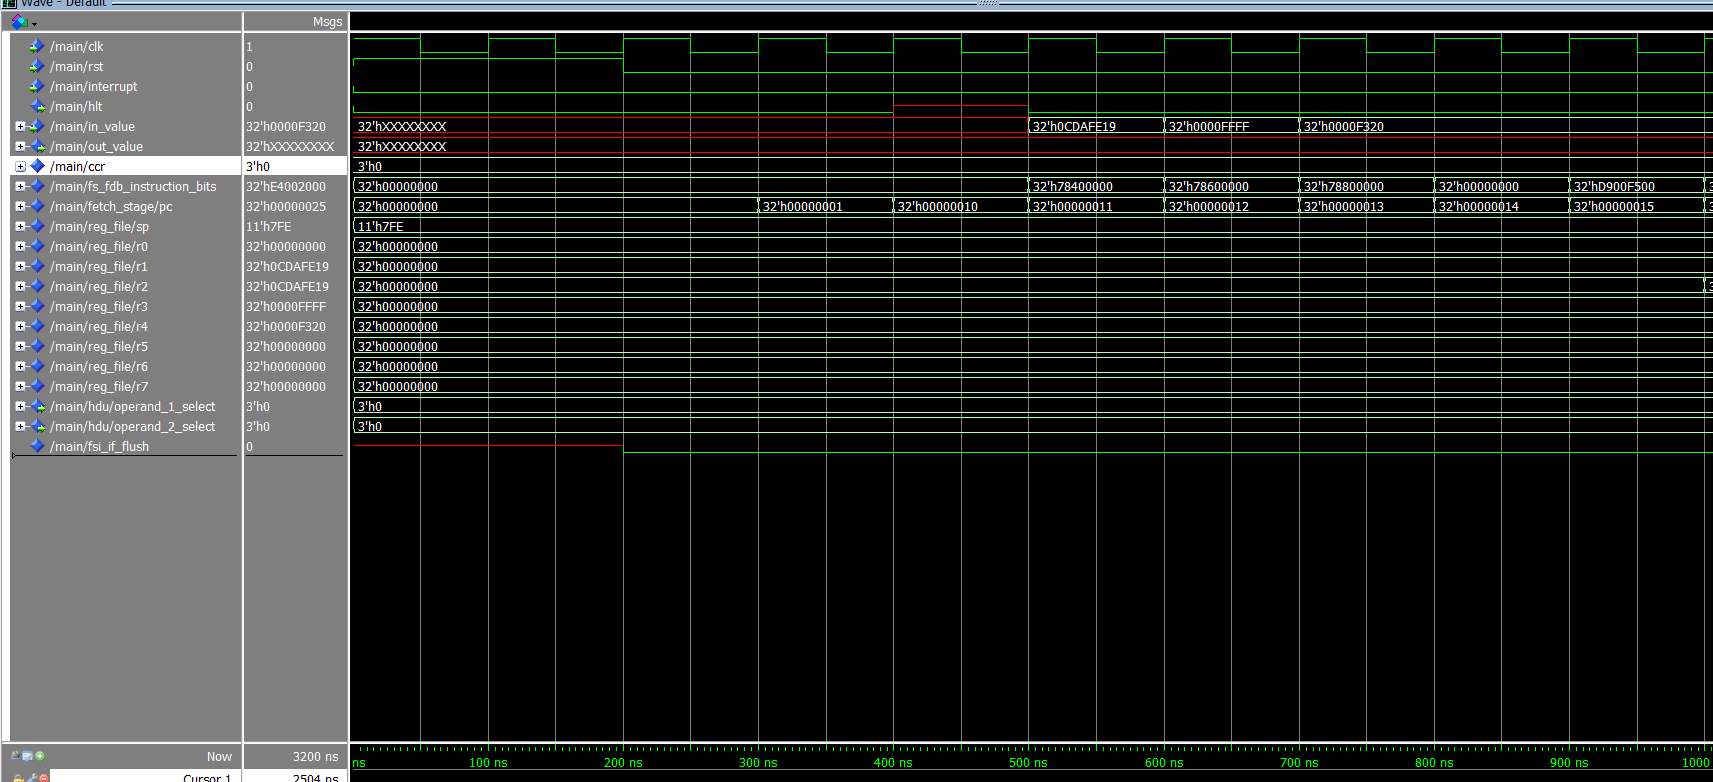
\includegraphics[width=0.9\textwidth]{images/test_cases/memory/Memory_no_stall_1.PNG}
    \caption{Memory No Forwarding Output wave 1}
    \label{fig:mem_no_1}
\end{figure}

\begin{figure}[H]
    \centering
    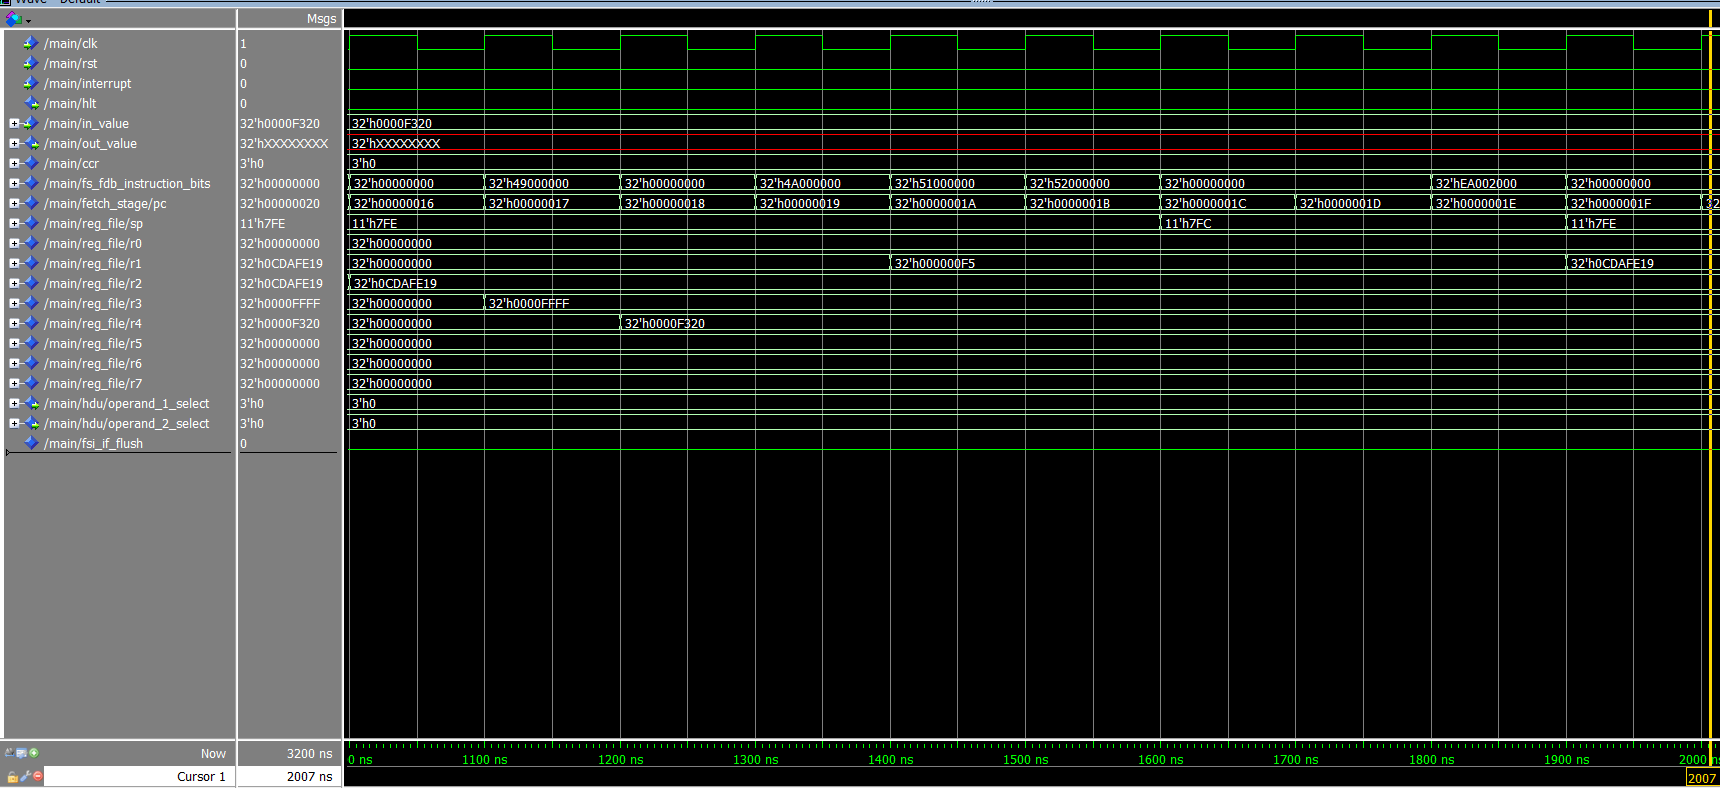
\includegraphics[width=0.9\textwidth]{images/test_cases/memory/Memory_no_stall_2.PNG}
    \caption{Memory No Forwarding Output wave 2}
    \label{fig:mem_no_2}
\end{figure}

\begin{figure}[H]
    \centering
    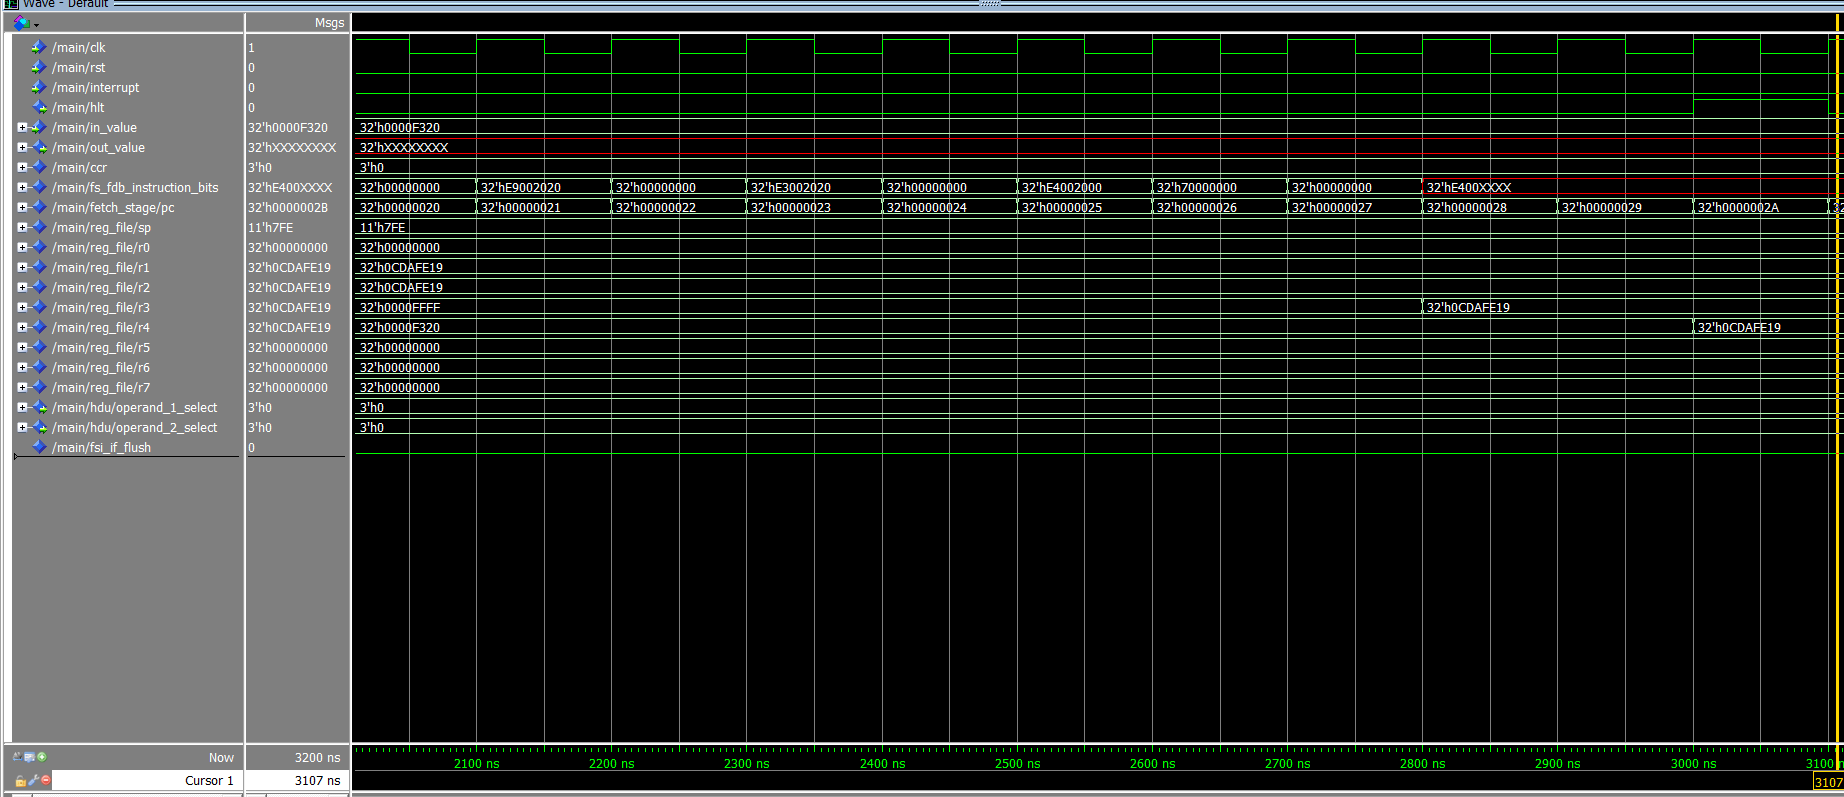
\includegraphics[width=0.9\textwidth]{images/test_cases/memory/Memory_no_stall_3.PNG}
    \caption{Memory No Forwarding Output wave 3}
    \label{fig:mem_no_3}
\end{figure}

\subsubsection{NOPs Solution}
The figures \ref{fig:mem_nop_1}, \ref{fig:mem_nop_2}, \ref{fig:mem_nop_3} and \ref{fig:mem_nop_4} show the output wave of code with NOPs solution.
\begin{figure}[H]
    \centering
    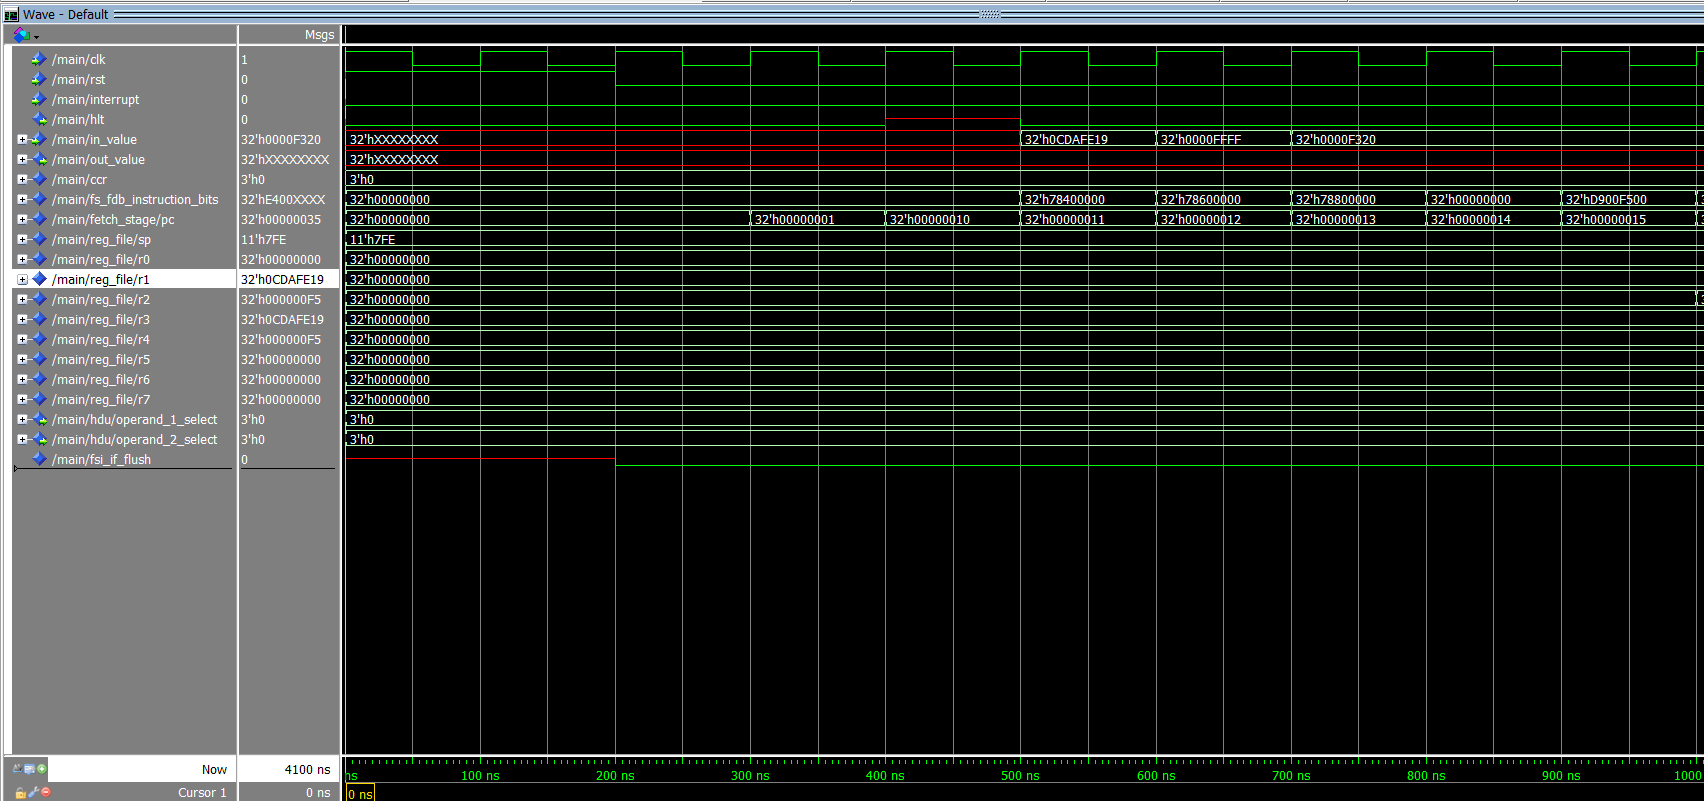
\includegraphics[width=0.9\textwidth]{images/test_cases/memory/Memory_NOP_1.PNG}
    \caption{Memory NOPs Solution Output wave 1}
    \label{fig:mem_nop_1}
\end{figure}

\begin{figure}[H]
    \centering
    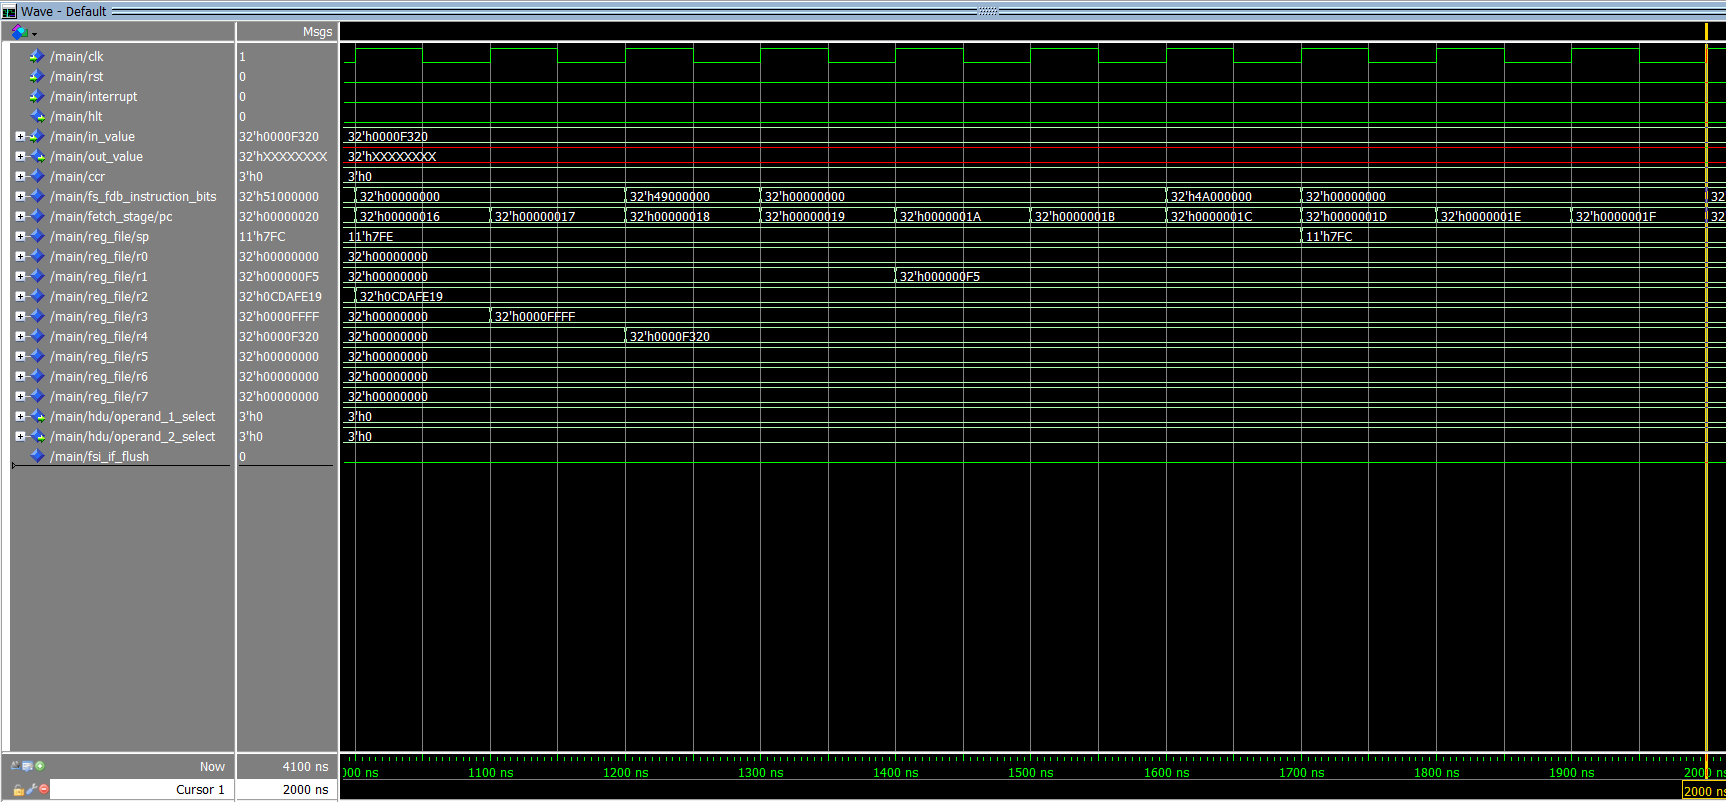
\includegraphics[width=0.9\textwidth]{images/test_cases/memory/Memory_NOP_2.PNG}
    \caption{Memory NOPs Solution Output wave 2}
    \label{fig:mem_nop_2}
\end{figure}

\begin{figure}[H]
    \centering
    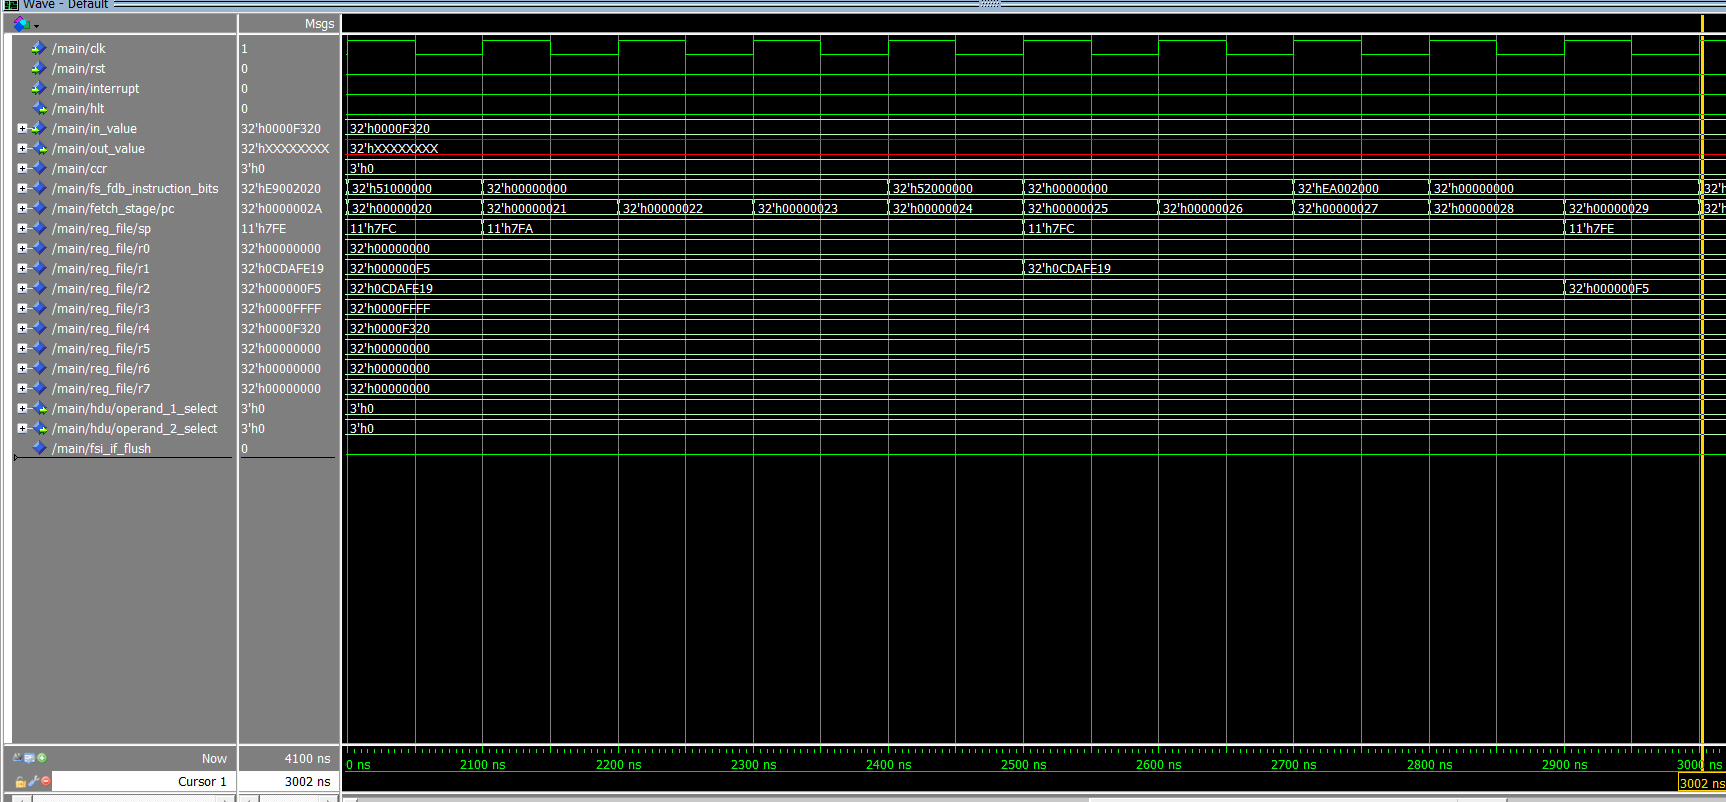
\includegraphics[width=0.9\textwidth]{images/test_cases/memory/Memory_NOP_3.PNG}
    \caption{Memory NOPs Solution Output wave 3}
    \label{fig:mem_nop_3}
\end{figure}

\begin{figure}[H]
    \centering
    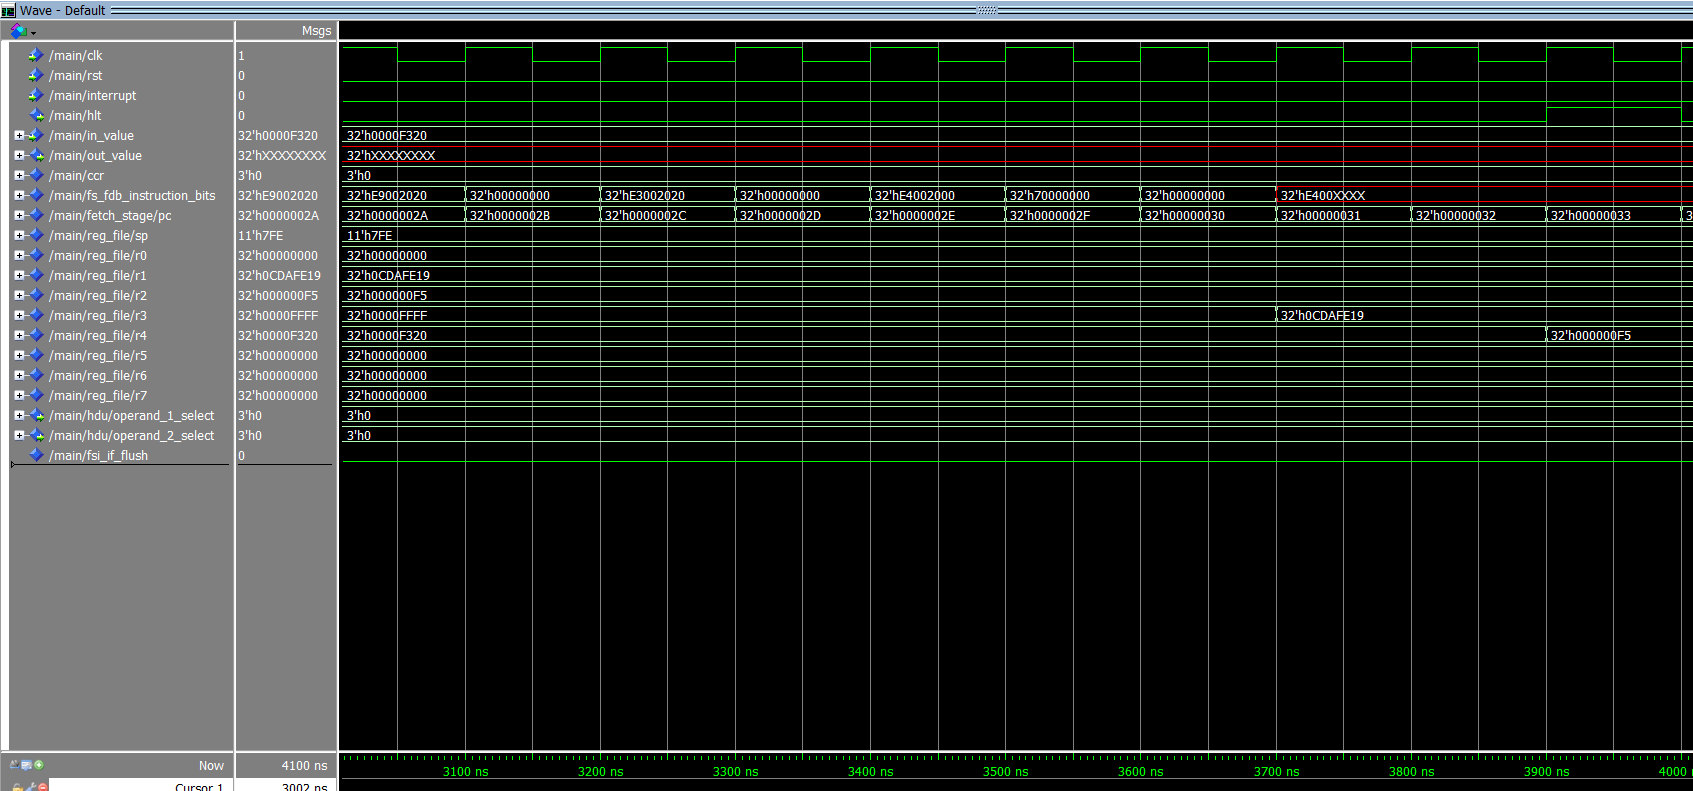
\includegraphics[width=0.9\textwidth]{images/test_cases/memory/Memory_NOP_4.PNG}
    \caption{Memory NOPs Solution Output wave 4}
    \label{fig:mem_nop_4}
\end{figure}

\subsection{Branch Test Case}

\subsubsection{Full Code}
The figures \ref{fig:br_reg_1}, \ref{fig:br_reg_2}, \ref{fig:br_reg_3}, \ref{fig:br_reg_4} and \ref{fig:br_reg_5} show the output wave of full code.
\begin{figure}[H]
    \centering
    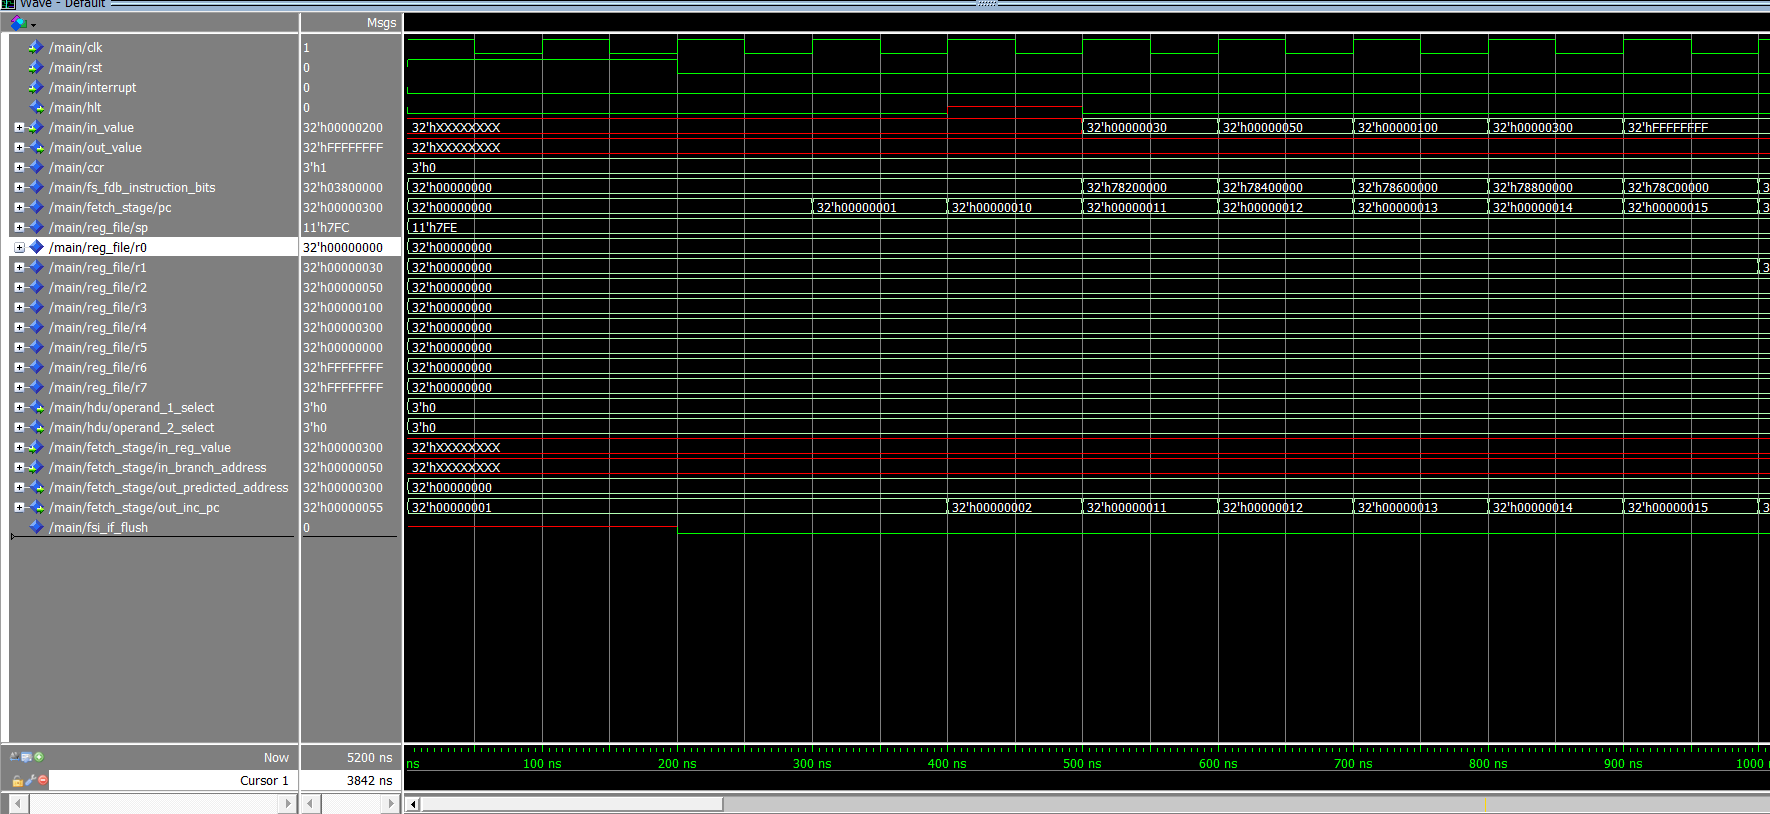
\includegraphics[width=0.9\textwidth]{images/test_cases/branch/Branch_regular_1.PNG}
    \caption{Branch Full Code Output wave 1}
    \label{fig:br_reg_1}
\end{figure}

\begin{figure}[H]
    \centering
    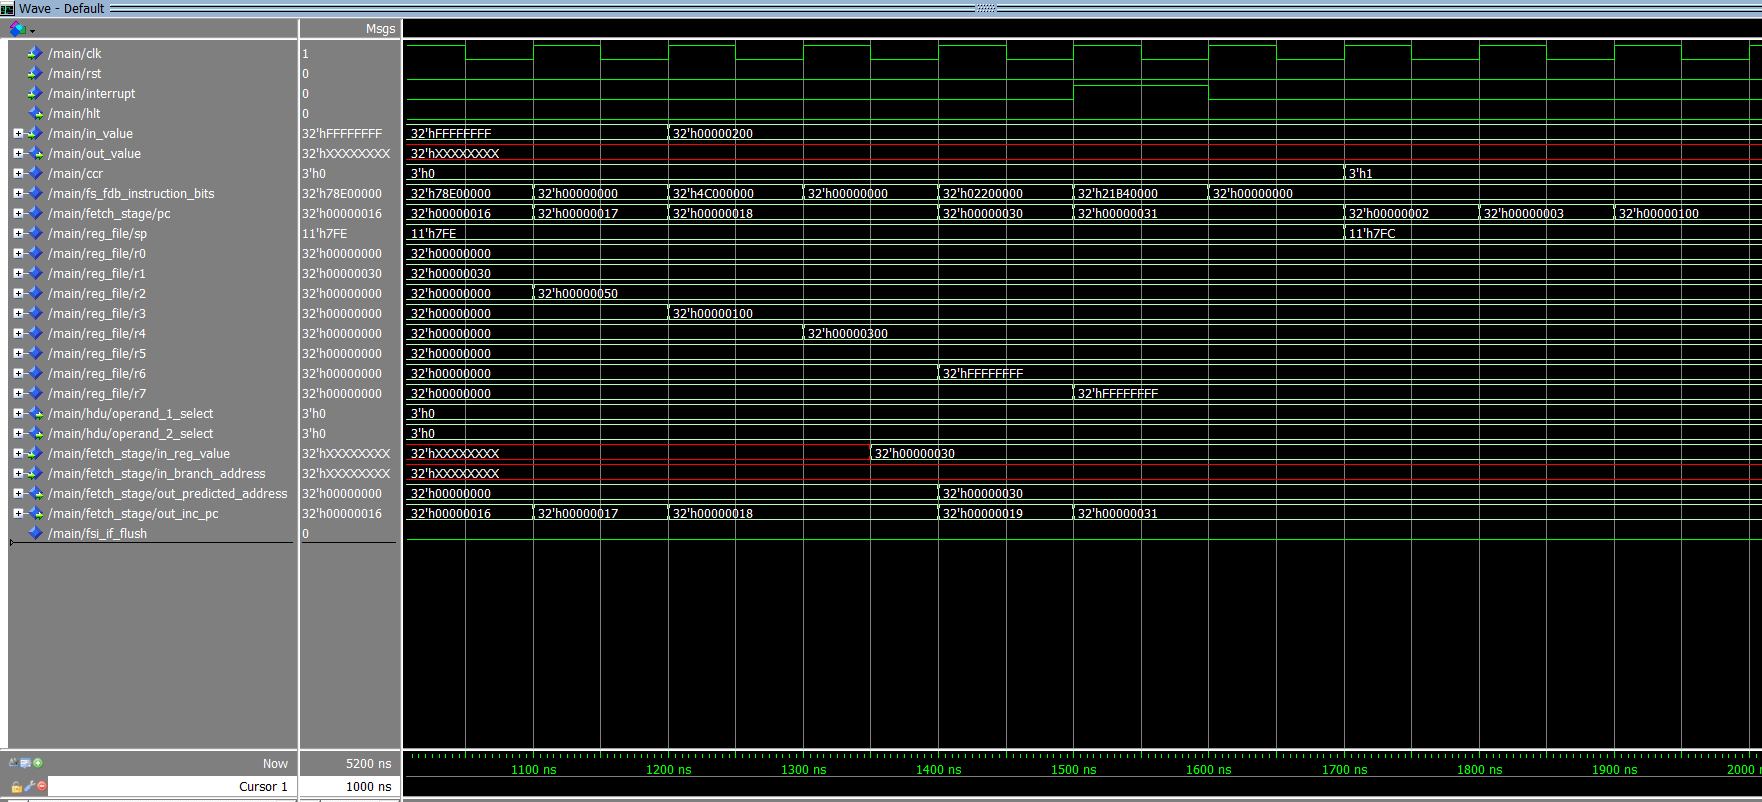
\includegraphics[width=0.9\textwidth]{images/test_cases/branch/Branch_regular_2.PNG}
    \caption{Branch Full Code Output wave 2}
    \label{fig:br_reg_2}
\end{figure}

\begin{figure}[H]
    \centering
    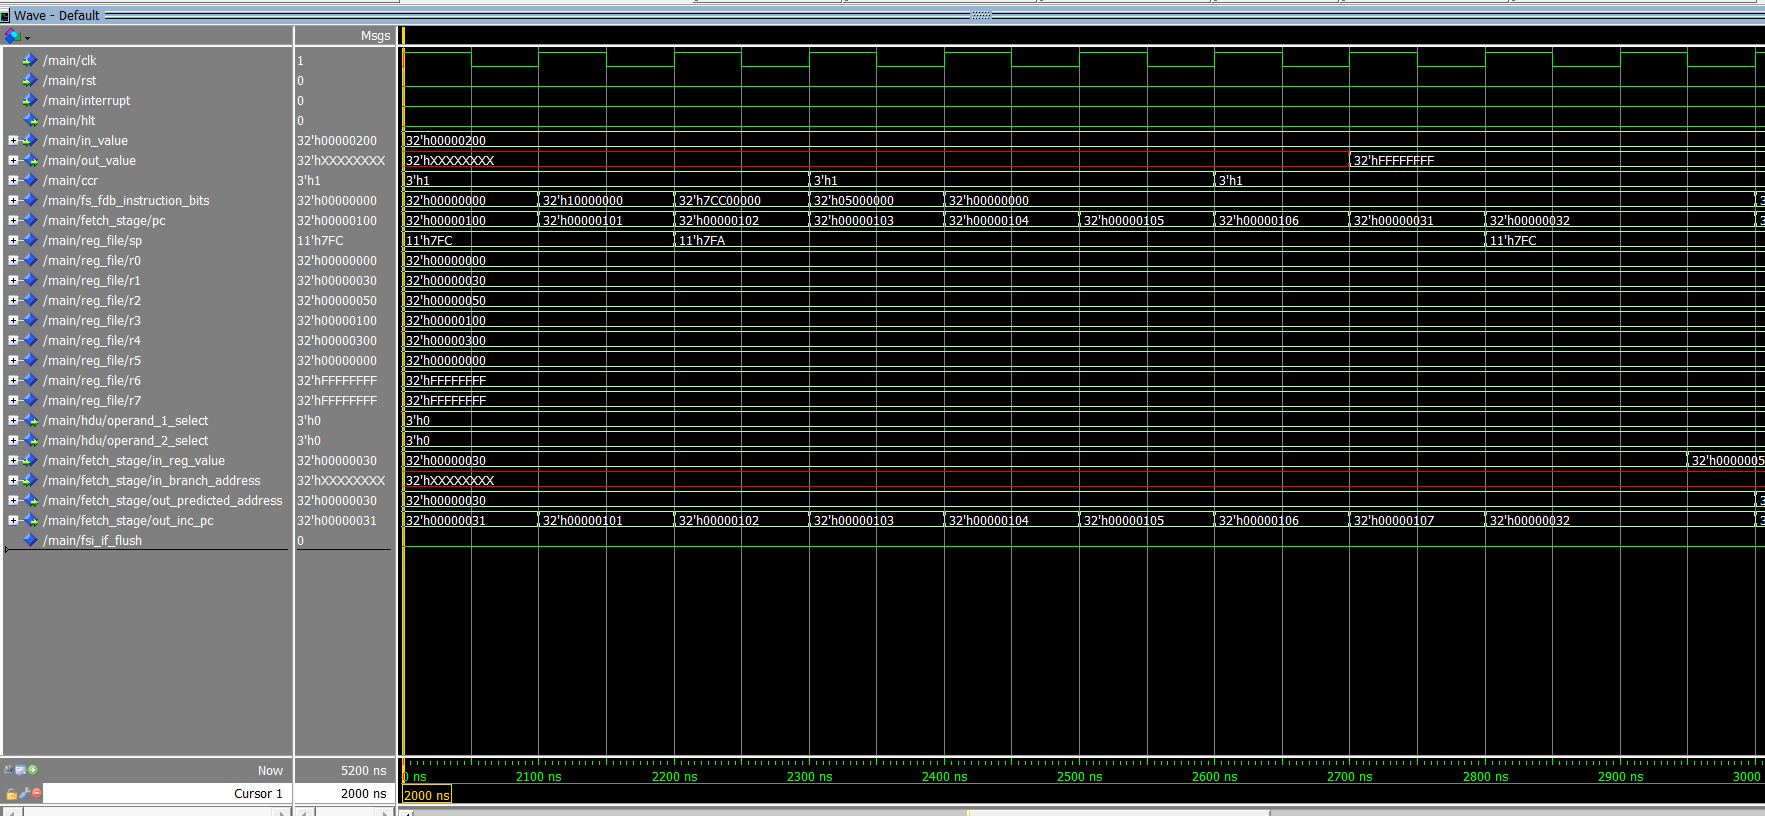
\includegraphics[width=0.9\textwidth]{images/test_cases/branch/Branch_regular_3.PNG}
    \caption{Branch Full Code Output wave 3}
    \label{fig:br_reg_3}
\end{figure}

\begin{figure}[H]
    \centering
    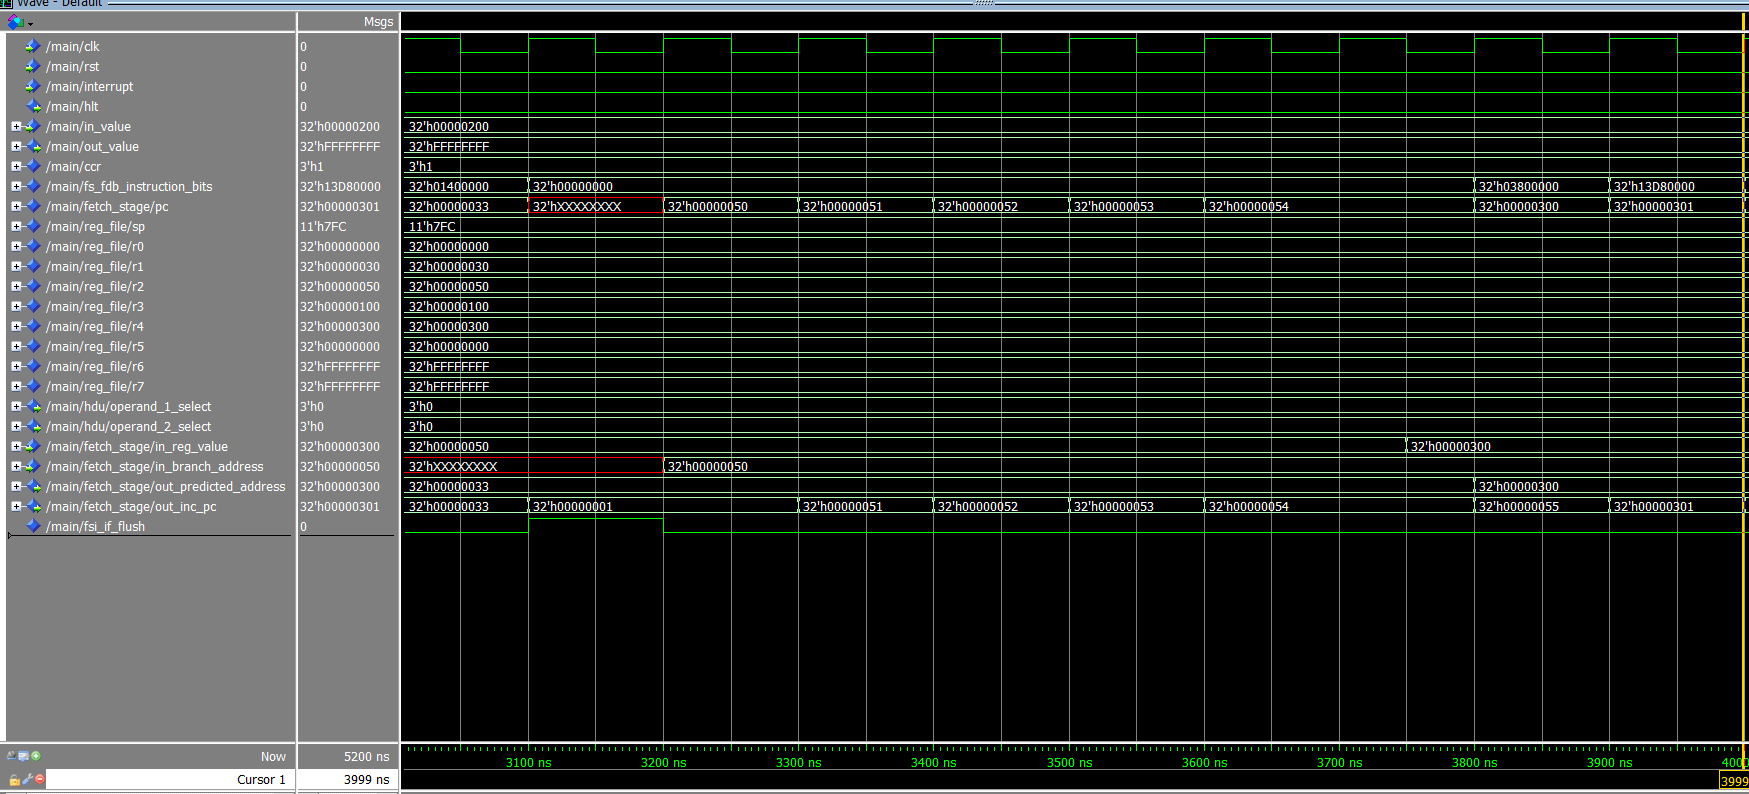
\includegraphics[width=0.9\textwidth]{images/test_cases/branch/Branch_regular_4.PNG}
    \caption{Branch Full Code Output wave 4}
    \label{fig:br_reg_4}
\end{figure}

\begin{figure}[H]
    \centering
    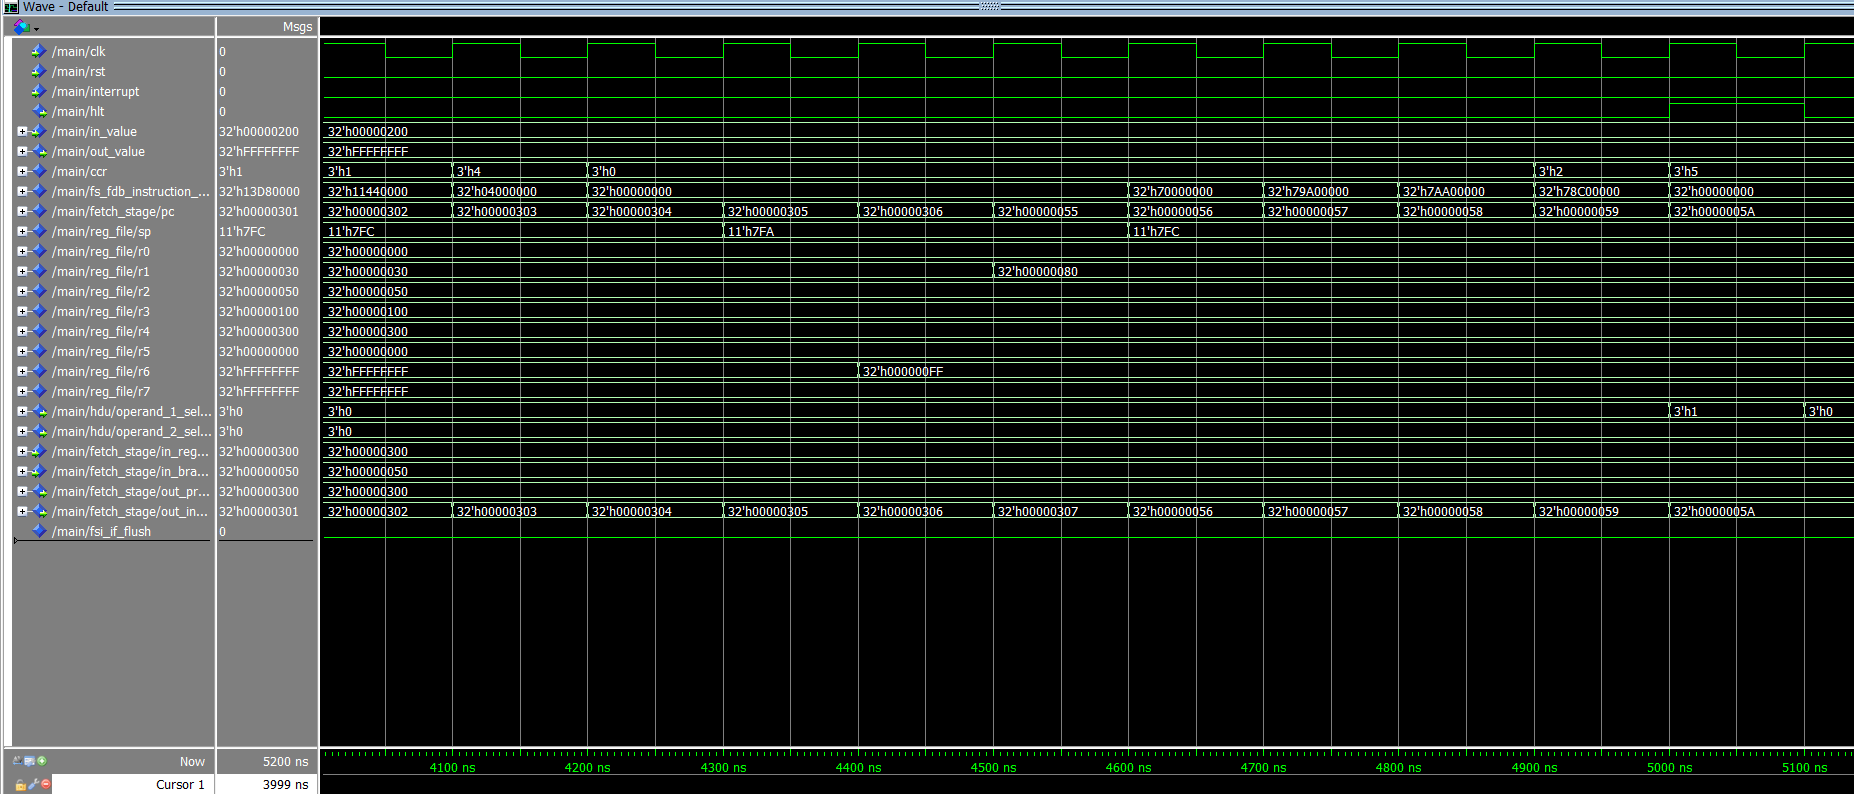
\includegraphics[width=0.9\textwidth]{images/test_cases/branch/Branch_regular_5.PNG}
    \caption{Branch Full Code Output wave 5}
    \label{fig:br_reg_5}
\end{figure}

\subsubsection{No Flush}
The figures \ref{fig:br_nop_1}, \ref{fig:br_nop_2}, \ref{fig:br_nop_3} and \ref{fig:br_nop_4} show the output wave of code with NOPs solution.
\begin{figure}[H]
    \centering
    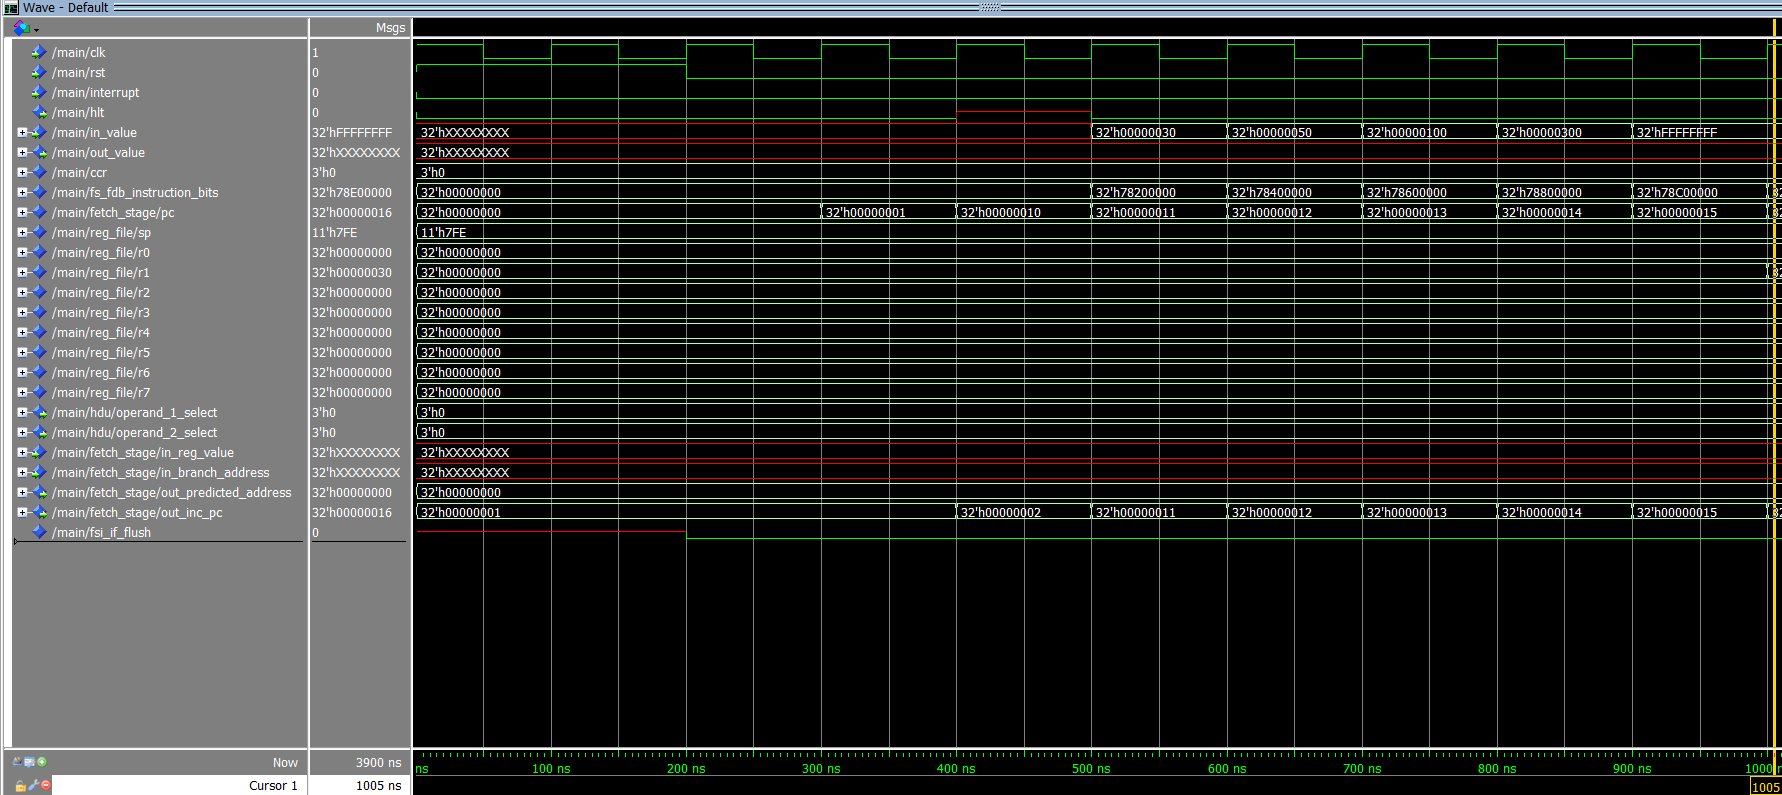
\includegraphics[width=0.9\textwidth]{images/test_cases/branch/Branch_no_flush_1.PNG}
    \caption{Branch No Flush Output wave 1}
    \label{fig:br_nop_1}
\end{figure}

\begin{figure}[H]
    \centering
    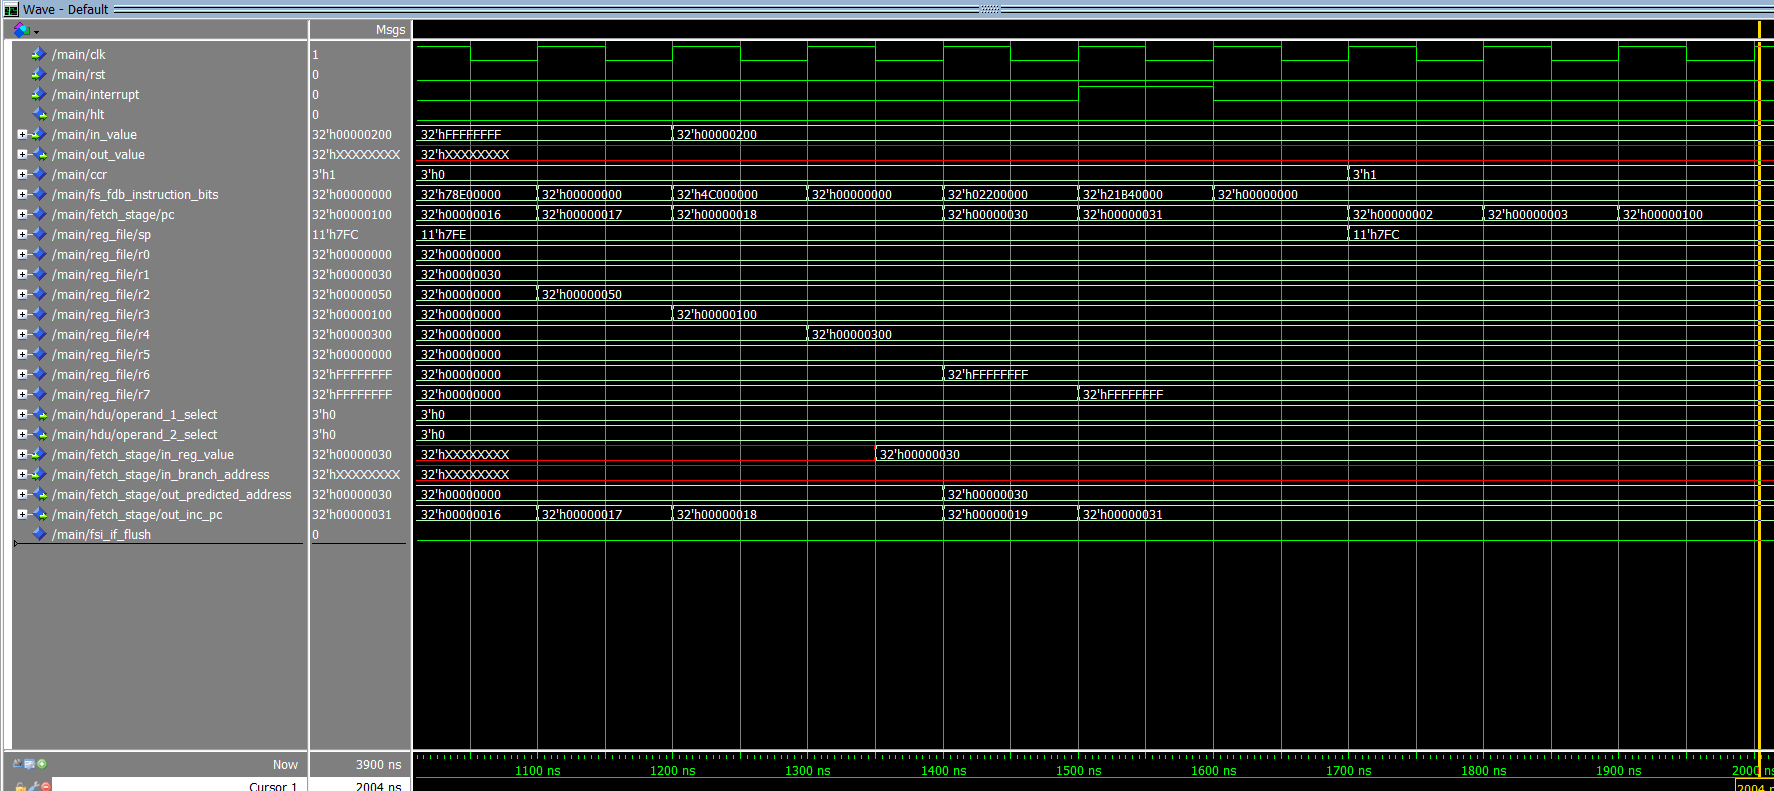
\includegraphics[width=0.9\textwidth]{images/test_cases/branch/Branch_no_flush_2.PNG}
    \caption{Branch No Flush Output wave 2}
    \label{fig:br_nop_2}
\end{figure}

\begin{figure}[H]
    \centering
    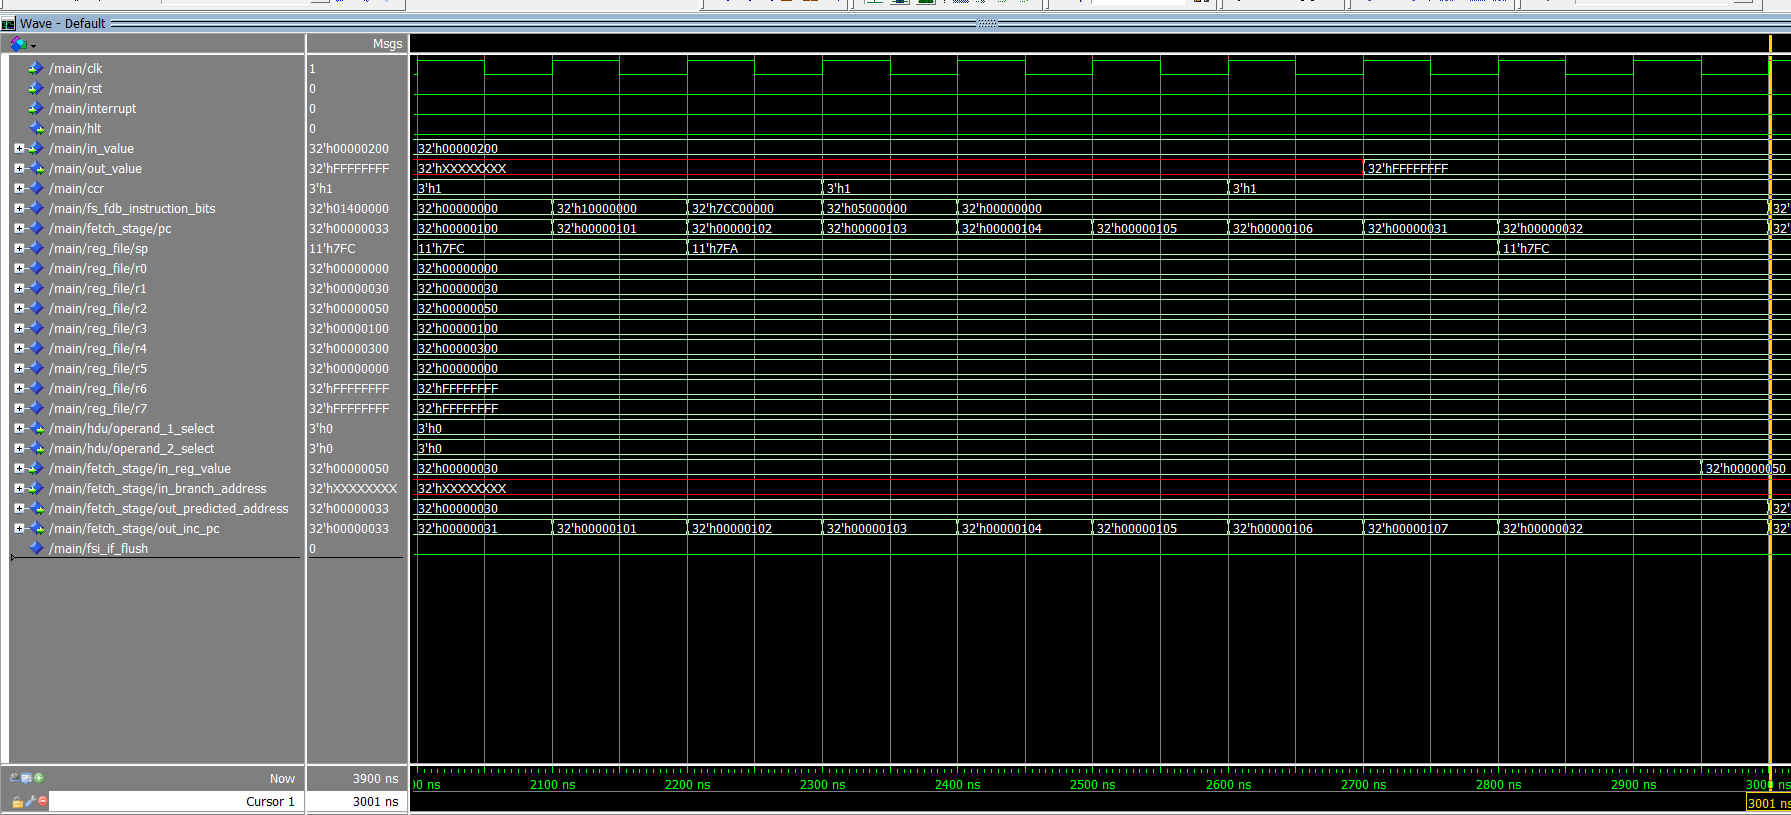
\includegraphics[width=0.9\textwidth]{images/test_cases/branch/Branch_no_flush_3.PNG}
    \caption{Branch No Flush Output wave 3}
    \label{fig:br_nop_3}
\end{figure}

\begin{figure}[H]
    \centering
    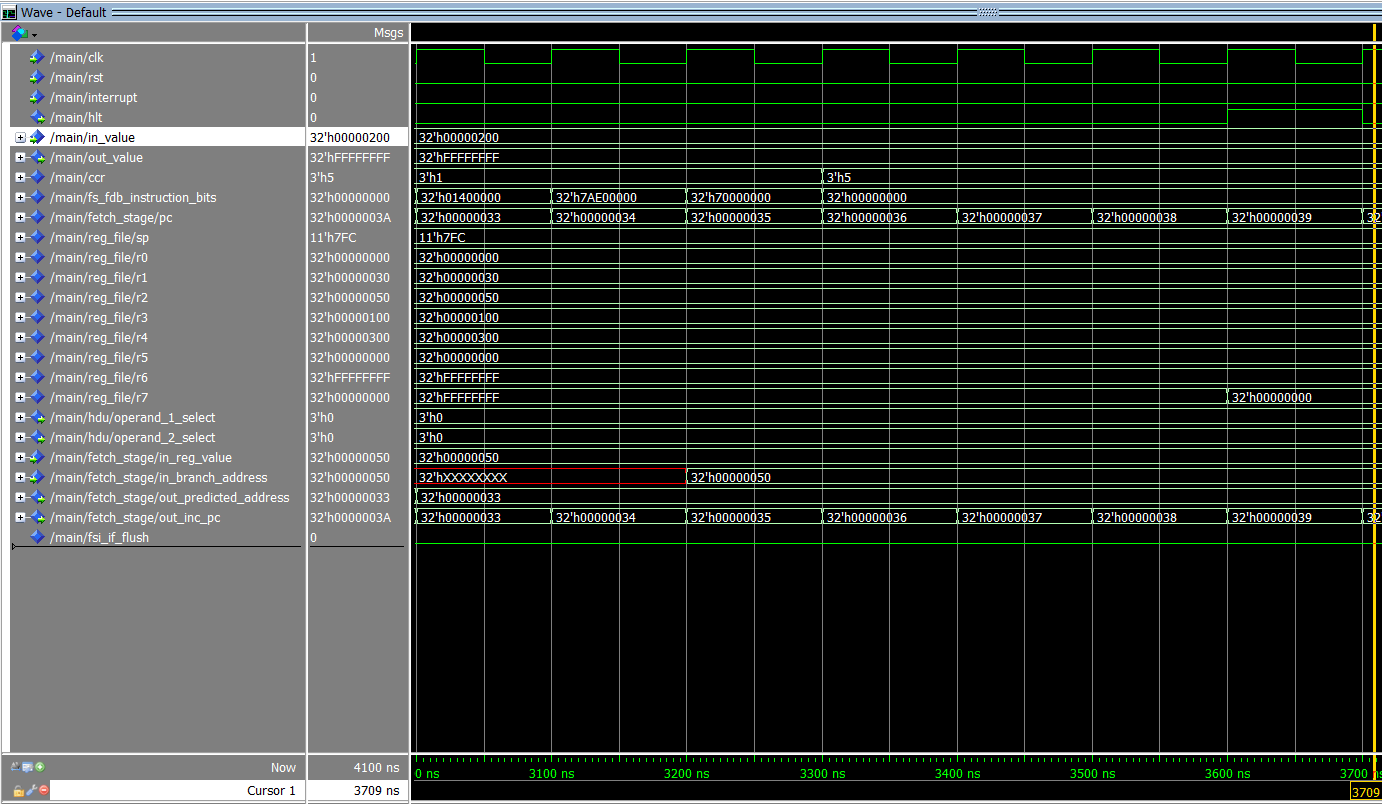
\includegraphics[width=0.9\textwidth]{images/test_cases/branch/Branch_no_flush_4.PNG}
    \caption{Branch No Flush Output wave 4}
    \label{fig:br_nop_4}
\end{figure}

\subsection{Branch Prediction Test Case}

\subsubsection{Full Code}
Since the branch prediction wave is too long, we will just add its ending. Full wave is included in submission files. The figures \ref{fig:brp_reg_1}, \ref{fig:brp_reg_2}, \ref{fig:brp_reg_3} and \ref{fig:brp_reg_4} show the output wave of full code.

\begin{figure}[H]
    \centering
    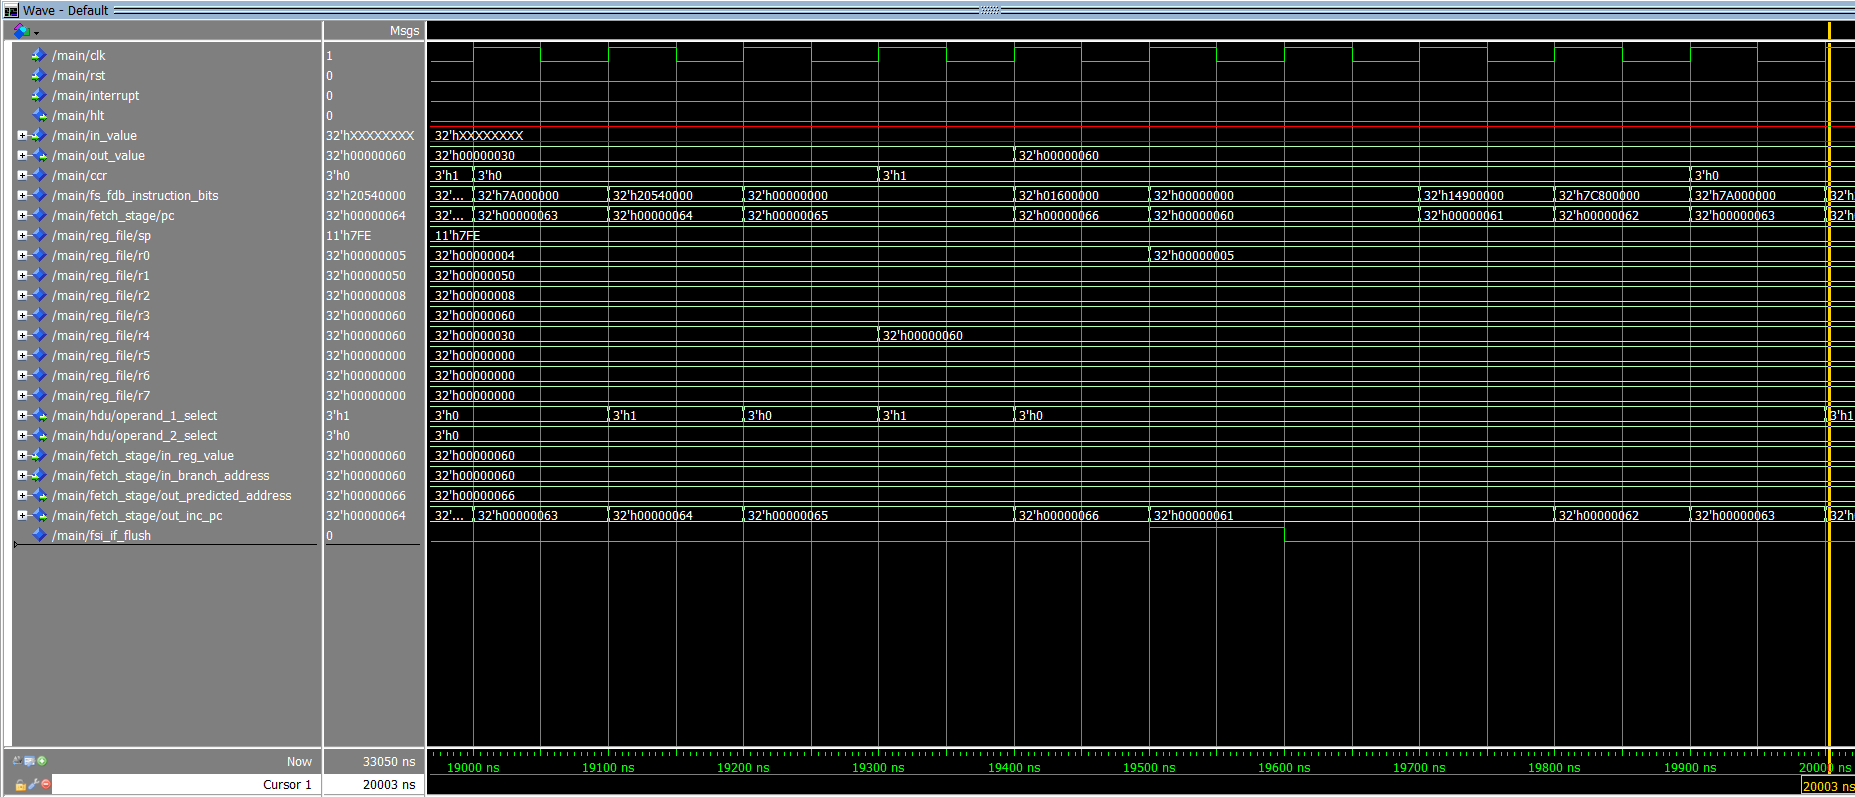
\includegraphics[width=0.9\textwidth]{images/test_cases/branch_prediction/BranchPrediction_regular_20.PNG}
    \caption{Branch Prediction Full Code Output wave 1}
    \label{fig:brp_reg_1}
\end{figure}

\begin{figure}[H]
    \centering
    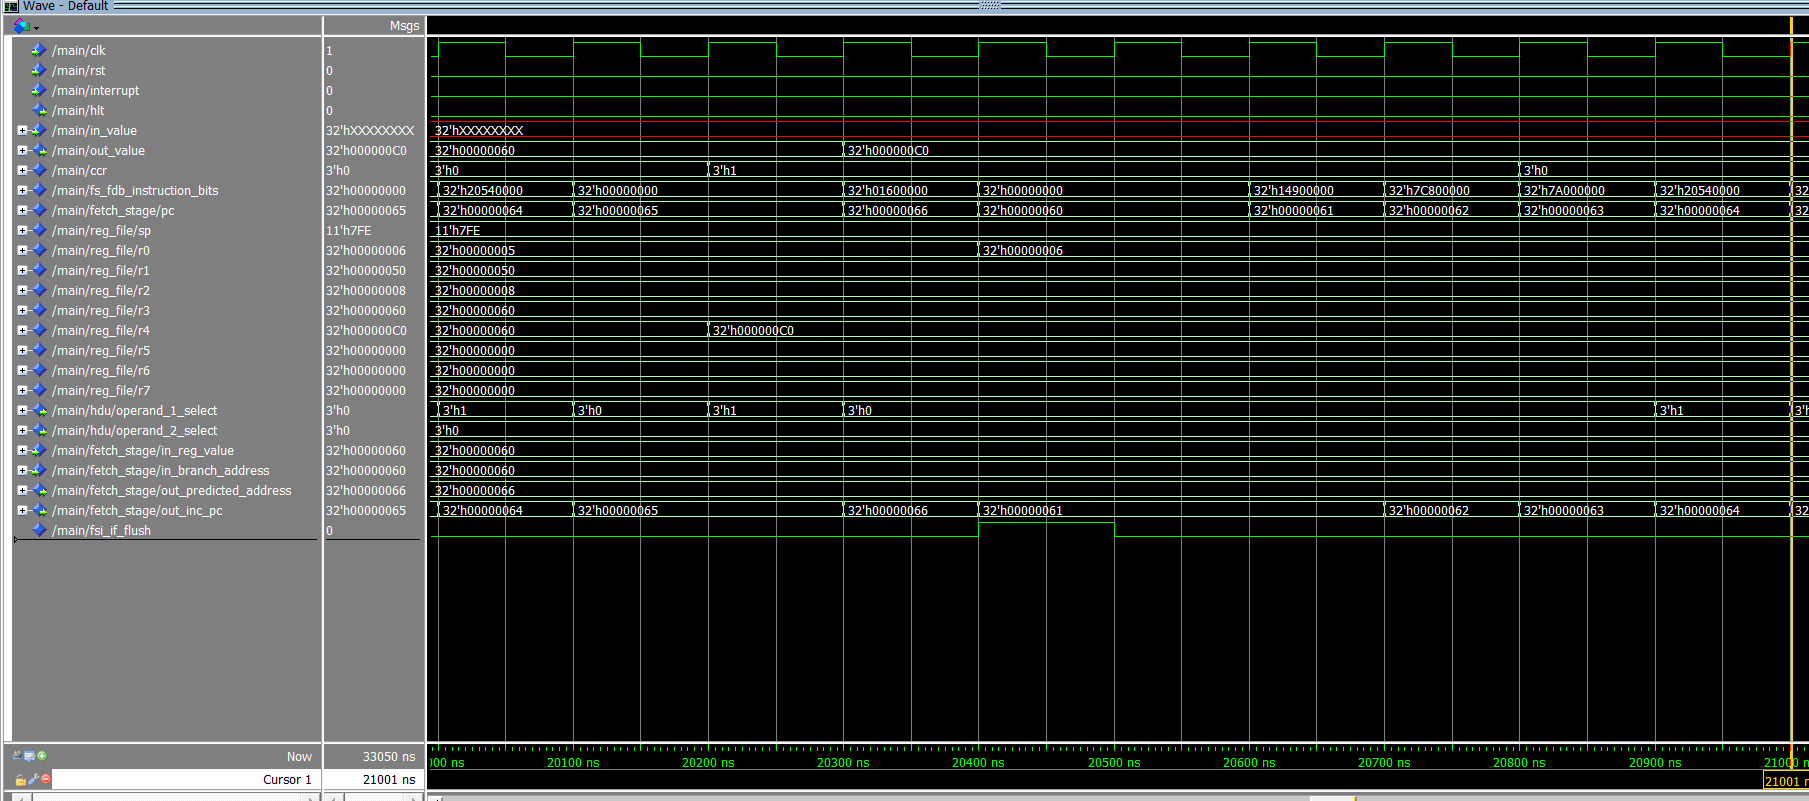
\includegraphics[width=0.9\textwidth]{images/test_cases/branch_prediction/BranchPrediction_regular_21.PNG}
    \caption{Branch Prediction Full Code Output wave 2}
    \label{fig:brp_reg_2}
\end{figure}

\begin{figure}[H]
    \centering
    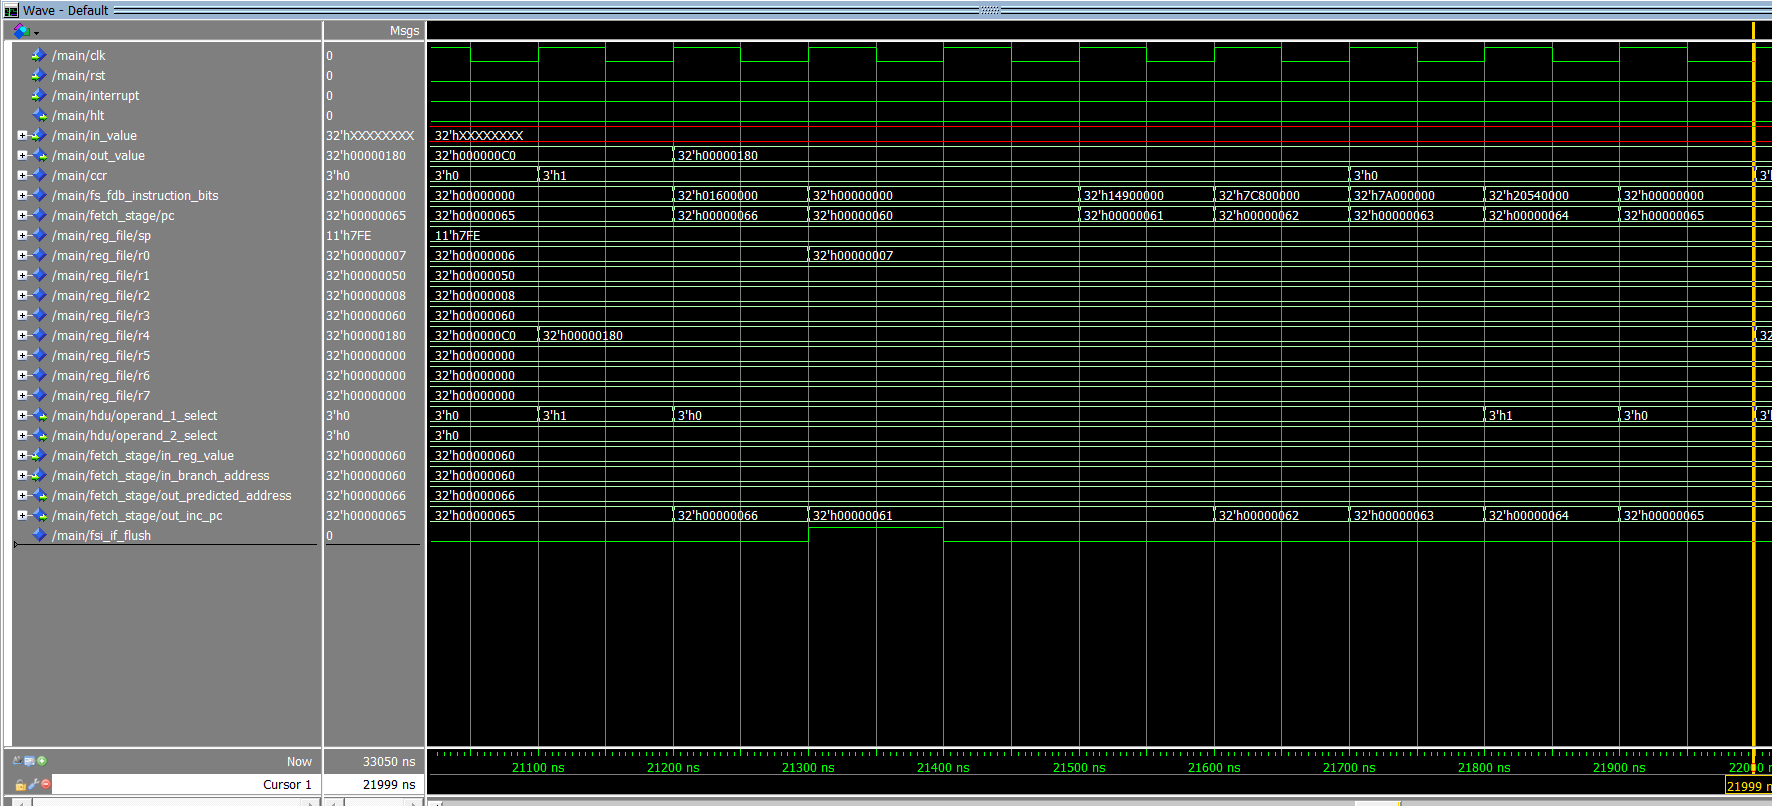
\includegraphics[width=0.9\textwidth]{images/test_cases/branch_prediction/BranchPrediction_regular_22.PNG}
    \caption{Branch Prediction Full Code Output wave 3}
    \label{fig:brp_reg_3}
\end{figure}

\begin{figure}[H]
    \centering
    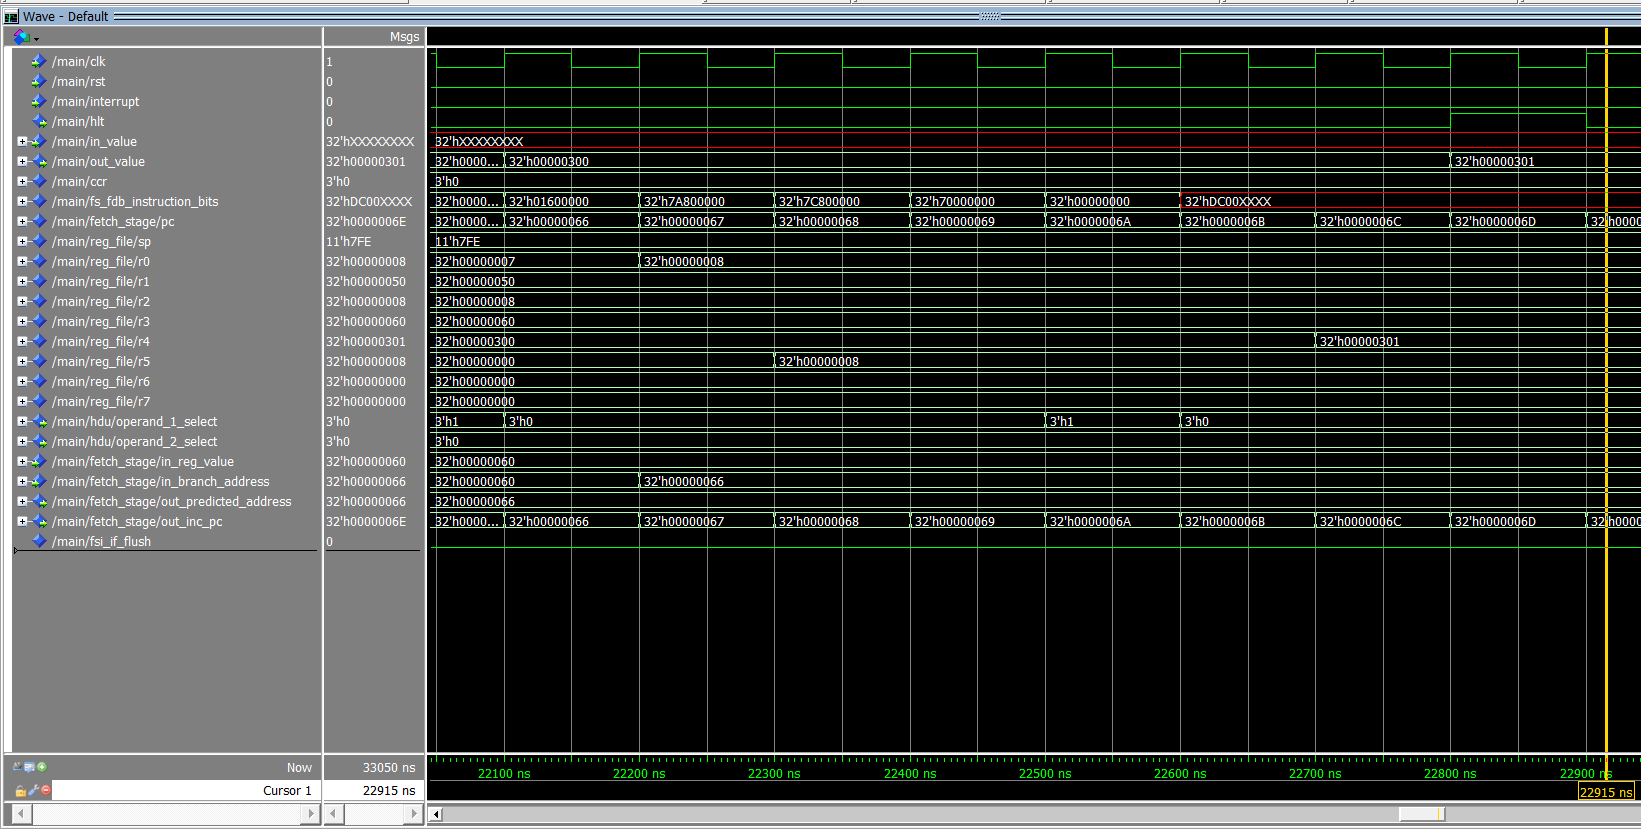
\includegraphics[width=0.9\textwidth]{images/test_cases/branch_prediction/BranchPrediction_regular_23.PNG}
    \caption{Branch Prediction Full Code Output wave 4}
    \label{fig:brp_reg_4}
\end{figure}

\subsection{Memory Cache Test Case}
Memory cache system is not implemented. 

\section{Complete Hazard Analysis}

\section{Hazard Detection Unit}

Disabling HDU can cause data hazards in consecutive instructions that uses same registers, also in instructions that uses the stack pointer. \\
We have shown the waves that illustrates the data hazards on the provided test cases. Also, we have shown that inserting NOPs between instructions that causes hazards can safely eliminate data hazards.

\section{Dynamic Branch Prediction}
The branch prediction occurs in fetch stage, which has no hazard handling. So, we count on decode stage to handle any possible problem in PC value. So, disabling branch prediction and flushing can cause wrong PC values that can't be adjusted. Consequently, that can cause infinite loops and wrong answers. \\
According to our design and implementation, this can't by solved by NOPs. So, the branch prediction should be enabled all the time.